\documentclass[12pt]{report}
\usepackage{ECE_Dissertation_Style}
\usepackage{amsmath,amssymb,latexsym,float,epsfig,subfigure,overpic}
%these margins allow you to use the default "shrink oversize pages" option when printing
\usepackage[lmargin=1.40 in, rmargin=0.86 in,tmargin=1.0 in,bmargin=1.0 in]{geometry}
\usepackage{indentfirst}
\usepackage{afterpage}
\usepackage{sectsty}
\usepackage{hyperref}
\usepackage{caption}
\usepackage{etoolbox}
\usepackage{mathrsfs}
\usepackage{booktabs}
\usepackage{breqn}
\usepackage[ruled]{algorithm}
\usepackage{algpseudocode}
\usepackage[per-mode=symbol, detect-weight=true, binary-units=true]{siunitx}
\usepackage{rotating}
\usepackage{tikz}
\newcommand{\figwid}{0.22\columnwidth}
\renewcommand{\d}[1]{\ensuremath{\operatorname{d}\!{#1}}}
\newcommand{\xupdownarrow}[1]{%
  {\left\updownarrow\vbox to #1{}\right.\kern-\nulldelimiterspace}
}
%%% bookmarks - color them black
\hypersetup{
	colorlinks=true,
	citecolor=black,
	filecolor=black,
	linkcolor=black,
	urlcolor=black
}
%Set graphics path
\graphicspath{{./pictures/pdf/},{./pictures/ps/},{./pictures/png/},{./pictures/jpg/}}
\captionsetup{format=hang}
%Fill pages with text and floats
\renewcommand\textfraction{.1}
\renewcommand\topfraction{.9}
\renewcommand\bottomfraction{.7}
\renewcommand\floatpagefraction{.7}
%Remove white space above chapter headings
\makeatletter
\patchcmd{\@makechapterhead}{\vspace*{50\p@}}{}{}{}% Removes space above \chapter head
\patchcmd{\@makeschapterhead}{\vspace*{50\p@}}{}{}{}% Removes space above \chapter* head
\makeatother


\begin{document}

%Set limits on font sizes for headings
\chapternumberfont{\fontsize{16}{20}\selectfont}
\chaptertitlefont{\centering\fontsize{16}{20}\selectfont}
\sectionfont{\fontsize{14}{16}\selectfont}
\subsectionfont{\fontsize{12}{14}\selectfont}

%%
%%
\title{Robotic Manipulators:
\protect\\Cryogenic Magnetic Manipulation System, Two-body magnetic manipulation, and Low-cost Robotic Manipulators} %% If you want to specify a linebreak
                               %% in the thesis title, you MUST use
                               %% \protect\\ instead of \\, as \\ is a
                               %% fragile command that \MakeUpperCase
                               %% will break!
\author{Benedict Isichei}
\department{Department of Electrical and Computer Engineering}

%% Can have up to four readers in addition to the advisor.
%% All have the form
%%
%%  \reader{Name}[Department][Institution]
%%
%% The second and third arguments are optional, but if you wish to
%% supply the third, you must supply the second. Department defaults
%% to the department defined above and Institution defaults to a blank.

\advisor{Dr. Aaron T. Becker, Assistant Professor}
\firstreader{Dr. David Mayerich, Assistant Professor}
\secondreader{Dr. Rose Faghih, Assistant Professor}
\thirdreader{Dr. Julien Leclerc, Postdoctoral researcher}
%\setcounter{secnumdepth}{2}
\degree{Master of Science}
\major{Electrical Engineering} 

\copyrighttrue
\copyrightyear{2018}
\submitdate{Aug 2018} % Must be the month and year of graduation,
                         % not thesis approval! As of 2010, this means
                         % this text must be May, August, or December
                         % followed by the year.

%defaults to thesis option
\dissertationfalse

%%%%%%%%%%%%%%%%%%%%%%%%%%%%%%%%%%%%%%%%%%%%%%%%%%%%%%%%%%%%%%%%%%%%%%%%%%%%%%%
% COVER PAGES:  Flyleaf, copyright page, title page, signature page
%
\makecoverpages

%%%%%%%%%%%%%%%%%%%%%%%%%%%%%%%%%%%%%%%%%%%%%%%%%%%%%%%%%%%%%%%%%%%%%%%%%%%%%%%
% ACKNOWLEDGMENTS
%
% Put acknowledgments in a file called "ack.tex" and it'll be inputted here.
\begin{acknowledgements}

% acknowledgements for thesis

I would like to thank Dr. Aaron Becker for his patience, advice and support while I was writing this. Thank Dr. Julien Leclerc and Dr. Shiva Shahrokhi for their patience and advice while I was working on their respective projects. I would also like to thank my Parents for their love, encouragement and support during the entire project. Lastly, I’m extremely grateful to the various members of the swarm robotics lab for being there when I had issues and having no problems stepping in with explanations. 
\end{acknowledgements}

%%%%%%%%%%%%%%%%%%%%%%%%%%%%%%%%%%%%%%%%%%%%%%%%%%%%%%%%%%%%%%%%%%%%%%%%%%%%%%%
% ABSTRACT
%
% Put abstract in a file called "abs.tex" and it'll be inputted here.
\abstitlep
\abstractsection

% abstract for thesis

%This is the abstract.  It has a limit of 150 words for a masters thesis and 350 words for a PhD dissertation.

In the field of robotics, there are various control systems utilized depending on the kind of robot being considered. This project presents three different robotic manipulators, and then compares their control systems. The first system is a cryogenic manipulation system. In this system, the robotic workspace is a 150mm3 cube, and the system implements a 3-dimensional control on the robot’s position and orientation. To obtain accurate results, and obtain higher torque without a solid Iron core, this system has all its coils cooled by liquid nitrogen to achieve a higher magnetic field without damaging the coils.  In the second system, a 2-directional position control method is implemented. This system is created to simulate wall contacts, and implement an algorithm for navigating magnetic robots in a cavity (2- dimensions in this case) given the constraints of the cavity’s geometry, and global inputs to the robots. The last system is a robotic manipulator created out of a toy robotic arm kit. The aim here was to increase the robot’s accuracy and augment its functionality, while making it userfriendly to students new to robotics.  

%%%%%%%%%%%%%%%%%%%%%%%%%%%%%%%%%%%%%%%%%%%%%%%%%%%%%%%%%%%%%%%%%%%%%%%%%%%%%%%
% TABLE OF CONTENTS
%
% print table of contents, figures and tables here.
\makecontentspages
%%

\prefacesection

%%%%%%%%%%%%%%%%%%%%%%%%%%%%%%%%%%%%%%%%%%%%%%%%%%%%%%%%%%%%%%%%%%%%%%%%%%%%%%%
% INSERT REAL CONTENT HERE
%
% Thesis Introduction

\chapter[Introduction]{Introduction}
\label{chap-intro}

Here begins the body of the thesis.





\chapter[A Magnetic Manipulator Cooled With Liquid Nitrogen]{A Magnetic Manipulator Cooled With Liquid Nitrogen}\label{chap-cryoMagnet}

This chapter is based on a Journal paper with Julien Leclerc, Benedict Isichei, and Aaron T. Becker.  My contribution was in the design of the heating elements interfacing the Manipulator and the robotic workspace, creating a camera mount for the system's sensory feedback, and working on the object tracking. 
Nathan Hui aided with editing the final version of the paper.


%%%%%%%%%%%%%%%%%%%%%%%%%%%%%%%%%%%%%%%%%%%%%%%%%%%%%%%%%%%%%%%%%%%%%%%%%%%%%%%%
\section{INTRODUCTION}
Magnetic actuation enables non-contact manipulation from a distance.  
This paper describes a magnetic manipulator, shown in Fig.~\ref{MagneticManipulatorPic}, that uses coils cooled by liquid nitrogen to reduce the size and power required to generate dynamic magnetic fields. 
Magnetic technologies have promise for several areas, including as actuation for minimally invasive surgery~\cite{Stereoaxis,nelson2010microrobots}.
Minimally invasive surgeries reduce patient recovery time, pain, and risks of infection~\cite{robinson2004minimally}. 
 These procedures are most often performed using a catheter, a tubular device that can access remote areas of the body through small incisions. 
  If all catheter actuation is applied at the proximal end, it is increasingly difficult to accurately control force and orientation of the distal tip as the length increases. 

% why magnetic actuation?  It already is being used!
 Magnetic actuation can be used to improve the effectiveness of minimally invasive surgeries. 
 The company Stereotaxis \cite{Stereoaxis} manufactures a magnetic system able to control the tip of a magnetic catheter and therefore increase the precision of the medical procedure. 
 The device uses two permanent magnets rotating around the workspace.
 \begin{figure}
	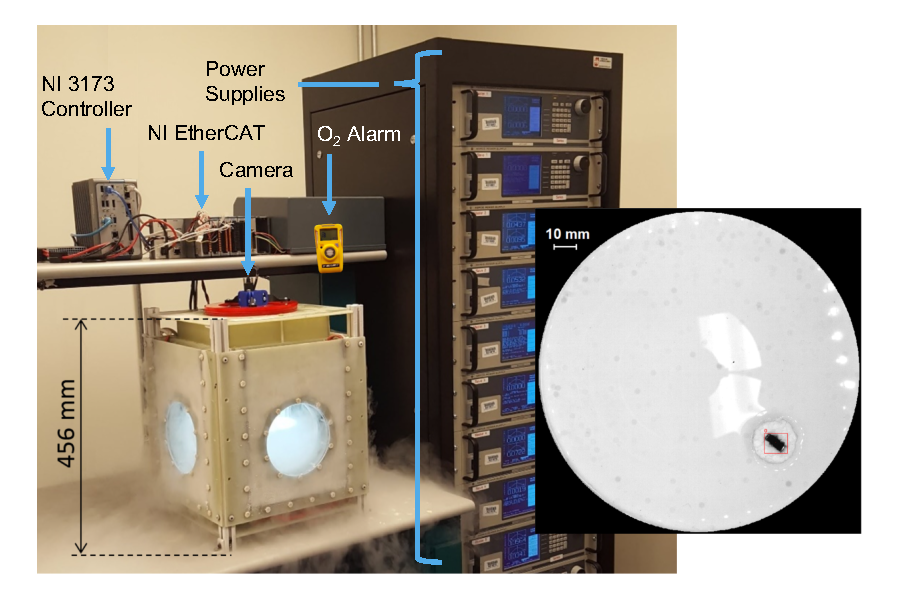
\includegraphics[width=\linewidth]{PictureManipulator.pdf}
	\caption{Picture of the magnetic manipulator while functioning. Inset shows view from the camera used to obtain position feedback of the robot.}
	\label{MagneticManipulatorPic}
\end{figure} 
 
 
 %As an example, coronary catheterization is a procedure consisting of inserting a catheter inside a blood vessel to access the coronary arteries. 
 Unfortunately, calcified fat deposits can build up inside arteries during the life of a person, a condition called atherosclerosis \cite{suri2010atherosclerosis}. 
 These deposits, called \emph{plaques}, may be detached by the friction between the catheter and the walls of the blood vessel and cause a stroke \cite{khatri2006ischemic,hamon2008periprocedural}.  
  \par
% Tetherless 
Tetherless magnetic robots could further decrease the invasiveness of procedures \cite{nelson2010microrobots}. 
The idea is to use external magnets to manipulate a small magnetic tool or capsule placed inside a patient. 
  The absence of tethers and the ability to navigate without touching the blood vessel walls \cite{kensicher2017towards} reduces the risk of plaque detachment. 
  A fast and accurate tracking method can enable precise control of the robot position during navigation. 
  However, permanent magnets are limited by their maximum rotational speed and acceleration and are therefore often unsuitable for fast dynamic control. 
 In contrast, electromagnets (EM) can generate magnetic fields with fast dynamics without moving parts. 
  Their magnetic field change rate is limited by either the power of the generator or the maximum voltage the magnet can sustain.
   \par
% About MRI
MRI scanners have EM and can be used as magnetic manipulators \cite{mathieu2006method, martel2007automatic, felfoul2016simultaneous}. 
 When a ferromagnetic piece (the robot) is placed inside this device, it becomes magnetized by the main magnetic field. 
  Because the main field is approximately uniform (less than 1 ppm of inhomogeneity \cite{wilson2002optimization}), it does not produce significant forces on the robot. 
  Instead, the MRI gradient coils can be used to produce a controlled force. 
 \par
 % Why MRI
The major advantage of using of MRI scanners for magnetic manipulation is that they are already widely available in hospitals and the robot's position can be tracked in real-time using the MR signal \cite{felfoul2009real, felfoul2016simultaneous}.
%the control is limited to three inputs as MRI scanners only have three sets of gradient coils. 
However, the large static magnetic field in an MRI permanently orients the magnetic field in the same direction, making torque control of robots impossible.
 The gradient coils can be used to generate forces on the robot.\par
% limitations on EMs
 Power consumption and heat dissipation are the primary limitations on EMs. 
 The current circulating inside a conductor produces Joule losses.
 Electromagnetic field strength is limited by its maximum power dissipation density. 
  More compact magnet designs can be achieved by reducing the amount of losses produced per unit of flux density. 
  If power consumption is not a concern, the maximum power dissipation density can also be increased.\par
 % discussion on ferromagnetic cores
Adding a ferromagnetic core to an EM is an effective way to increase the magnetic field and the forces produced without increasing the losses.
 Cores enable increasing the inductance value which in turn increases the total flux produced per ampere. 
 However, the use of a ferromagnetic core requires a closed bore geometry for the magnet. 
 This is often an issue for medical applications. 
  MRIs are designed with open bores on two opposite sides to accommodate the patient. 
 Additional openings could allow medical staff to access the patient during the procedure and decrease feelings of claustrophobia.\par    
 % Advantages of LN2
Using liquid nitrogen (LN2) is another way to decrease the amount of losses produced per unit of flux density. 
This method decreases the value of the electrical resistivity of copper and therefore allows more current to circulate inside the magnet for a given amount of losses. 
Cooling the EM to cryogenic temperatures offers another advantage: because the temperature of the coolant is low, the maximum safe temperature increase of the coil is larger. 
LN2 cooling therefore increases the maximum power dissipation density. 
LN2 is cheap (approximately 0.13 USD/Liter) and available in industrial quantities. 
It is non-toxic as gaseous nitrogen composes 78\% of the volume of our atmosphere. However, if large quantities of liquid nitrogen are evaporated, the level of oxygen in the room might decrease. An adapted ventilation system and a low oxygen alarm must be used to prevent anoxia. \par
% Outline
This paper presents the design and test of a magnetic manipulator cooled with LN2. 
A demonstration system is described in \S\ref{sec:System}.
The motivations and technical difficulties associated with this type of cooling are discussed in \S\ref{sec:CoolingWithLN2}.
A method to perform inverse magnetic calculations is then explained in \S\ref{sec:invMagnetics}.
 A robot trajectory controller is described in \S\ref{sec:TrajectoryControl}. 
 Next the system singularities are analyzed for 3-DOF control of a permanent magnet in \S\ref{sec:singularities}. 
  Experimental results are presented and analyzed in \S\ref{Experiment}. The paper concludes with lessons learned in this study.\par

%%%%%%%%%%%%%%%%%%%%%%%%%%%%%%%
\section{System Presentation}\label{sec:System}
The magnetic manipulator in Fig.~\ref{MagneticManipulatorPic} is designed to fit a human heart phantom. 
Detailed build instructions, a bill of materials, and CAD models are available\footnote{\href{https://github.com/RoboticSwarmControl/magnetic-manipulator-l2n-source}{github.com/RoboticSwarmControl/magnetic-manipulator-l2n-source}}.
The working volume is a sphere with radius 0.075 m. % $\SI{0.75}{\metre}$.
The system is composed of six copper coils arranged in a cubical shape (see Fig. \ref{CAD}). 
   Each coil is placed and held in an independent cryostat. 
 The cryostats contain the LN2 and were built using G10. 
 G10 is a fiberglass-epoxy composite able to withstand cryogenic temperatures. 
 Ordinary plastics become brittle at cryogenics temperatures, but G10 remains resilient. 
 G10 is also electrically nonconductive, an important feature to avoid induced currents.
 Induced currents generate a magnetic field that opposes variations in the applied field, making the system less responsive.
 Induced currents also generate heat.
%Induced currents generate a field that opposes the changing magnetic field.
\par
% induced currents oppose the changing magnetic field
% 
\begin{figure}
	%\includegraphics[width=\linewidth]{cadimage.png}
	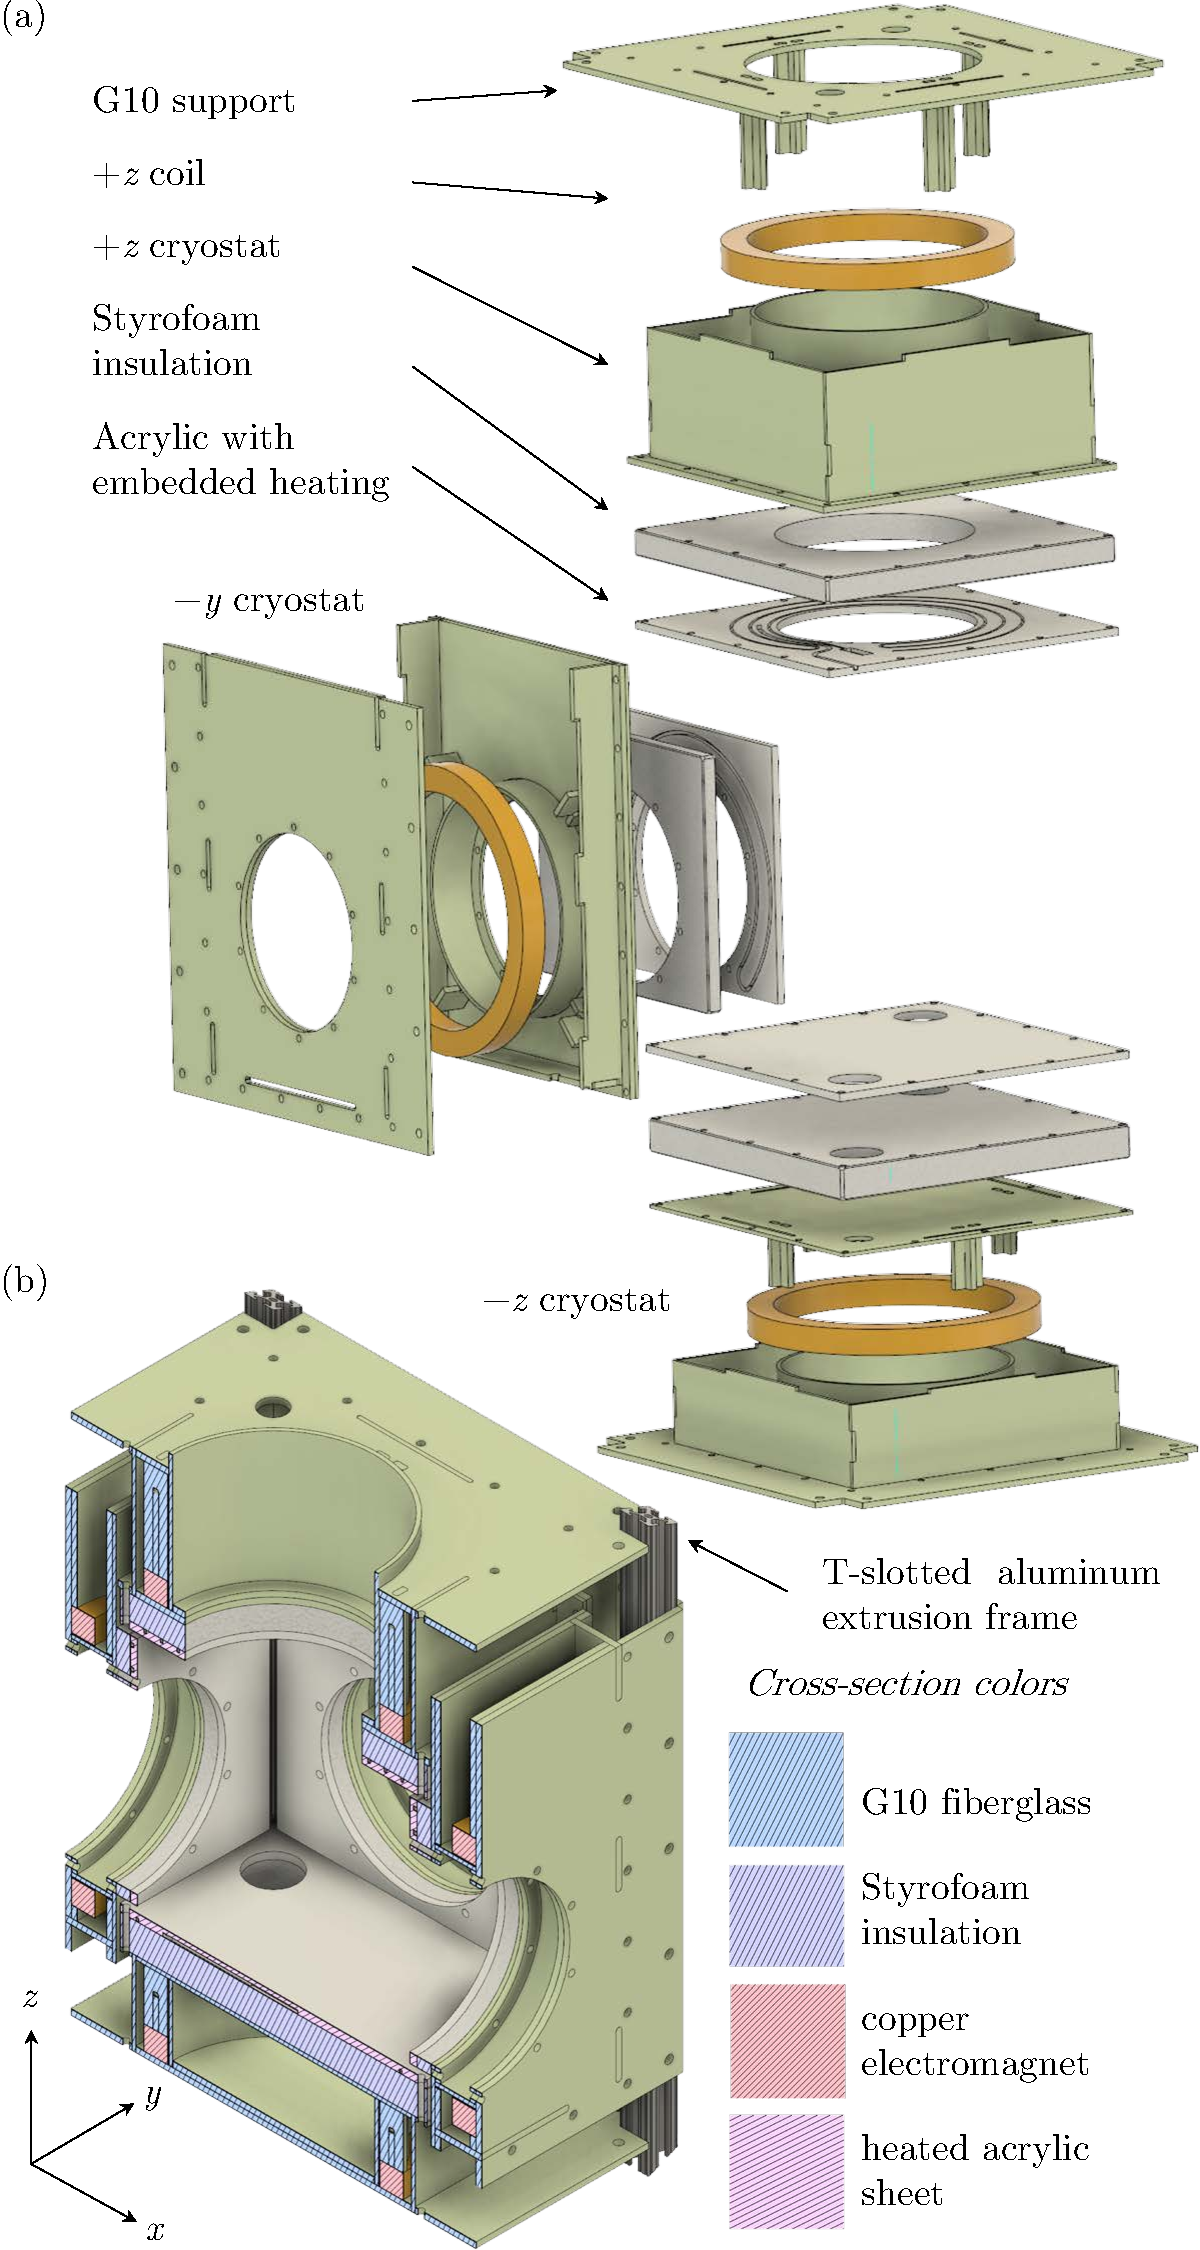
\includegraphics[width=.7\linewidth]{Fig2exploded2sm.pdf}
	\caption{CAD model of the magnetic manipulator: (a) exploded view of three cryostats, (b) cross-section view.}
	\label{CAD}
\end{figure}
 Uninsulated G10 walls become cold and water present in air condenses and freezes on them. 
  This ice could interfere with objects in the workspace. 
  To prevent icing, the cryostat walls facing the workspace are insulated by a  10 mm thick layer of Styrofoam insulation.  %$\SI{10}{\milli\metre}$
Six acrylic plates (one for each internal face) containing a resistive heater and a  thermocouple temperature sensor cover the inner face of the insulation.
  The temperature of the internal walls surrounding the workspace are regulated using a real-time controller.
The evaporation rate  of LN2 is the product $\mathscr{L}\cdot P_o$,  where $\mathscr{L}$ is the latent heat of vaporization, equal to 200 kJ/kg for LN2 and $P_o$ is the power dissipated. The maximum power consumption of each coil of the system is 2 kW. 
At maximum power, 0.74 liters of LN2 evaporate per minute.
%  (2*10^3  J)/s*(60 s)/min*(1 kg)/(200*10^3  J)*1L/0.807kg = 0.74 L/min
 \par
%
\begin{figure*}[ht]
\centering
	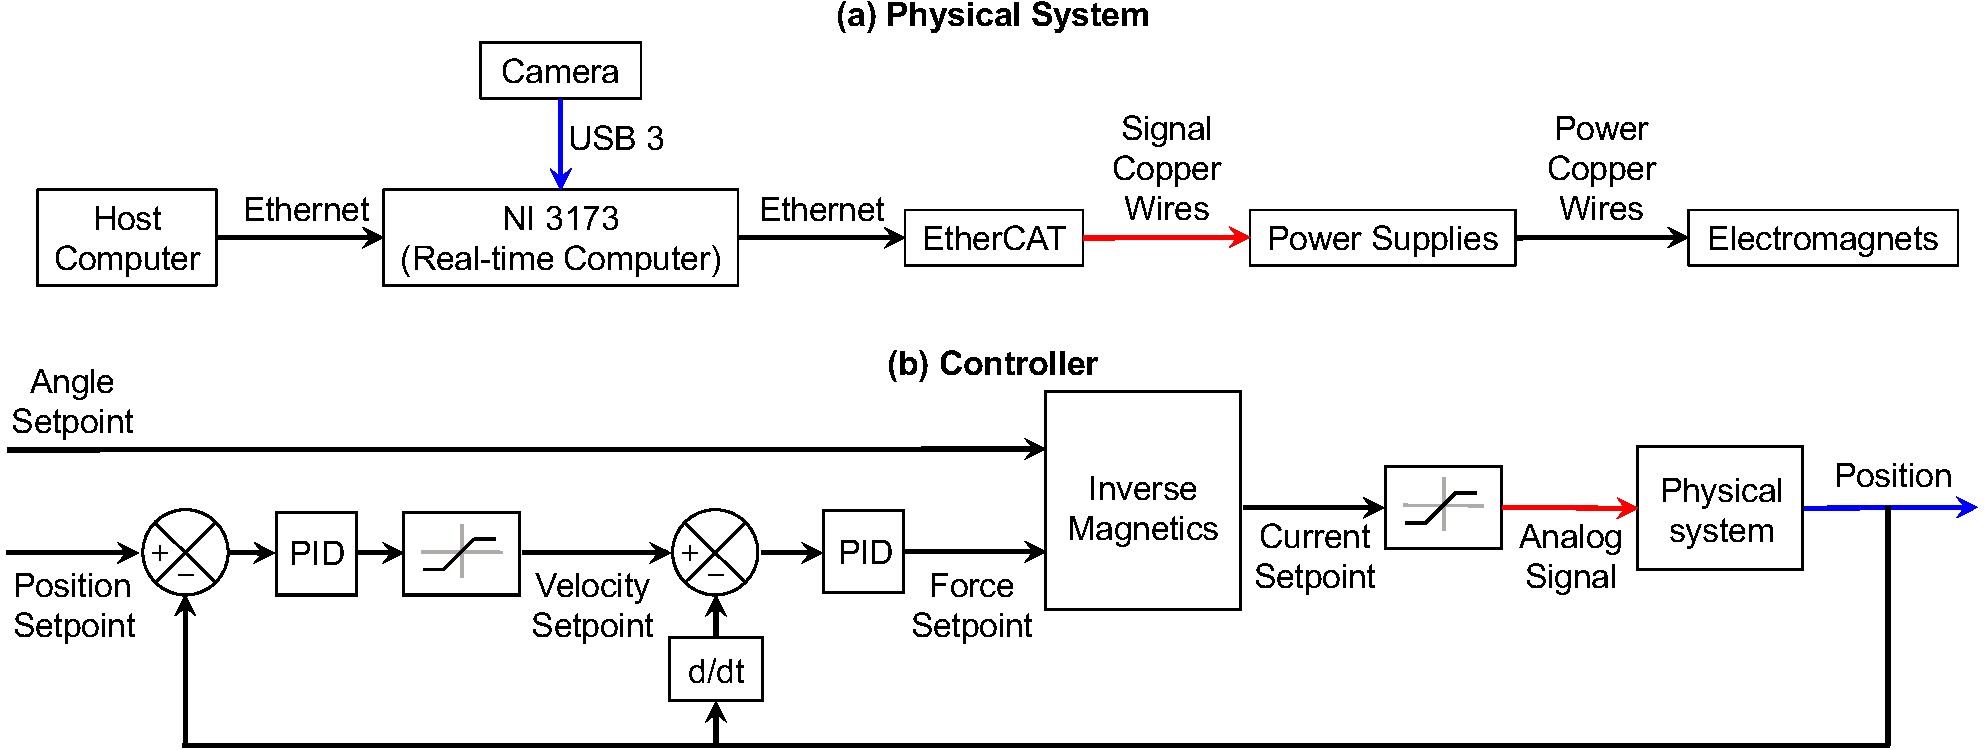
\includegraphics[width=\linewidth]{FigureController.pdf}
	\caption{Block diagram of (a) the physical hardware and (b) the controller used for position control.
	\label{fig:Controller}	}
\end{figure*}
%
12 Kepco BOP 20-50 generators power the system. Each power supply can generate 20 A under 50 V. %$\SI{20}{\ampere}$ under $\SI{50}{\volt}$. 
 Each coil is powered by two of these supplies connected in series. Each coil can, therefore, receive a maximum of 20 A under 100 V. %$\SI{20}{\ampere}$ under $\SI{100}{\volt}$.
 Each set of power supplies is controlled via an analog input. 
 While the current inside an EM is directly proportional to the magnetic flux density produced, the voltage applied on an EM is proportional to the time derivative of the flux density. 
 It is therefore easier to control the produced magnetic field by controlling the current rather than the voltage on the EM. 
 The BOP power supplies can do this when controlled in current mode. 
 In this mode, the power supplies output a current proportional to an analog input.

An industrial controller IC-3173 from National Instrument is used for real-time computation, as shown in Fig.~\ref{fig:Controller}(a).
 A set of two Basler acA2040 cameras are attached at orthogonal faces of the magnetic manipulator. 
  These cameras are used to obtain robot position and orientation in real-time (100 Hz). 
   Two high precision NI 9263 analog modules are used to generate the analog signal controlling the power supplies.
   
   The laboratory is equipped with a low oxygen alarm (Honeywell BW Clip, approximately 140 USD).

\section{Cooling with Liquid Nitrogen}\label{sec:CoolingWithLN2}
\subsection{Motivations}
The voltage $U_l$ at the terminals of a resistive coil can be calculated using the following equation:
\begin{equation}
U_l=L\cdot\frac{\d I(t)}{\d t}+R(t)\cdot I(t),
\label{Ul}
\end{equation}
where $I$ is the current in the coil, $L$ is the coil inductance, and $R$ is the coil resistance.
Two components are present in this equation:
\begin{itemize}
\item The term $L\cdot \d I(t)/ \d t$ is related to the magnetic energy change rate. This term does not cause losses if a four quadrant power supply is used. This type of power supply has the ability to transfer stored magnetic energy back to the electrical network. It is desirable to maximize $L\cdot \d I(t)/ \d t$ because a high magnetic energy change rate generates a large force change rate, a desirable feature for robot control. 
\item The term $R(t)\cdot I(t)$ is associated with Joule losses. It is an undesirable term for two reasons. First, it causes the coil to heat and decreases the energy efficiency of the system. Secondly, power supplies are limited by their maximum voltage. The voltage across the coil is shared between the two terms of equation \ref{Ul}. If the term $R(t)\cdot~I(t)$ is increased, less voltage is available for the term $L\cdot \d I(t)/ \d t$. LN2 cooling allows reducing the value of $R(t)$ by 87\%;
\end{itemize}
%As shown in subsection \ref{Forward}, the force produced on a permanent magnet is proportional to the magnetic flux density. However, 
The magnetic flux $\Phi$ produced by a solenoid is proportional to its inductance as shown in \eqref{flux}. In \cite{kummer2010octomag}, the authors use a ferromagnetic core to increase the value of $L$ and therefore increase the amount of force generated. LN2 cooling is different and increases the generated field by increasing the value of $I(t)$.
\begin{equation}
\Phi (t)=L\cdot I(t)
\label{flux}
\end{equation}
  It is technically difficult to scale up magnetic manipulators \cite{kummer2010octomag}. 
  Air-cooled human-size manipulators would use comparitively large electromagnets to produce the magnetic field.
  This technical challenge could potentially be solved using LN2 cooling.  
  This type of cooling enables a significant decrease in the system price, size, mass and/or improve its energy efficiency. \par
  %
  This tendency is illustrated in Fig.~\ref{fig:ComparisonMagnetsDesigns} and Table \ref{DesignsCompare}, which compares the flux density magnitude produced by different EM designs along their revolution axis. 
 The comparison was computed using the magnetic modeling software Finite Elements Method Magnetics (FEMM \cite{meeker2010finite}).
 EM1 and EM3 correspond to the EM present in our experimental setup when respectively cooled with LN2 (EM1) and forced air (EM3).  
 The gain of flux density and magnetic gradient when cooling with LN2 is +435\% and is relatively equal to the gain in current (see Table \ref{CoolingComparison}). 
 EM2 and EM4 correspond to the same EM as 1 and 3 except that ferromagnetic cores were added to each. 
 The gain in flux density is small, approximately 10\%. 
 EM6 is a forced-air-cooled EM with a ferromagnetic core designed to generate the same magnetic field as EM1.  
  EM6 must be $2.5\times$ longer than EM1. 
  EM5 is the same as EM6 except that the ferromagnetic core was removed. 
  The relative gain in flux density obtained by adding a ferromagnetic core is larger for EM5 and EM6, suggesting that the gain is related to the aspect ratio of length/diameter of the coil.


%The amount of current that can circulate inside an EM is limited by its temperature. If the temperature become two high, the insulating wire will burn. Insulating varnishes are available in different classes depending on the maximum temperature tehy can withstand. For exemple, plain enamel is a class A insulator and can withstand a temperature of 378K. 
%The density of power released via Joule heating in a wire is equal to dP=rho.J2.dV with rho being the electric resistivity, J the current density and dV an infinitesimal volume element. The electrical resistivity of conducting materials varies a lot with temperature. At room temperature (300K) copper has an electrical resitivity of ??? ohm/m. When cooled at liquid nitrogen temperature (77K), it decreases to ??? ohm/m, approximately 7.7 times smaller. Accordinegely to eq. ?, if the electrical resistivity is divided by 100 then the current density must be multiplied by 10 to produce the same amount of losses. In other words, a copper EM working at a current I at room temperature can safely be operated at 10*I when cooled with LN2 as no more losses are produced. In practice, this value can be further increased because the coil will be able to tolerate more losses before damages appear. Indeed, the working temperature is lower and a larger temperature variation is therefore available before damages appear. In addition, the heat exchange coefficient is larger when cooling with LN2 compared to air.


%
\begin{table*}[ht]
\centering
%
\centering
\caption{Description of the electromagnet designs compared in Fig.~\ref{fig:ComparisonMagnetsDesigns}.}
\label{DesignsCompare}
\scalebox{0.8}{
\begin{tabular}{@{}lcccccc@{}}

\toprule
Electromagnet ID                    & 1               & 2               & 3          & 4          & 5  & 6        \\ \midrule
%Internal radius  $R_i$        & 90 mm          & 90 mm          & 90 mm     & 90 mm     & 90 mm & 90 mm    \\
External radius $R_e$         & 110 mm          & 110 mm          & 110 mm     & 110 mm     & 110 mm & 110 mm    \\
Coil width  $T_r$        & 20 mm          & 20 mm          & 20 mm     & 20 mm     & 20 mm & 20 mm    \\
Coil length  $T_z$                   & 20 mm           & 20 mm           & 20 mm      & 20 mm      & 50 mm & 50 mm     \\
Number of turns            & 795             & 795             & 795        & 795        & 1987 & 1987      \\
Copper wire                & AWG 22          & AWG 22          & AWG 22     & AWG 22     & AWG 22  & AWG 22    \\
Core                       & Air             & Hyperco-50      & Air        & Hyperco-50 & Air & Hyperco-50\\
Cooling method             & LN2 & LN2 & Forced air & Forced air & Forced air & Forced air \\
Max. cont. current & 7.5 A           & 7.5 A           & 1.4 A      & 1.4 A      & 1.4 A & 1.4 A \\
Schematic & 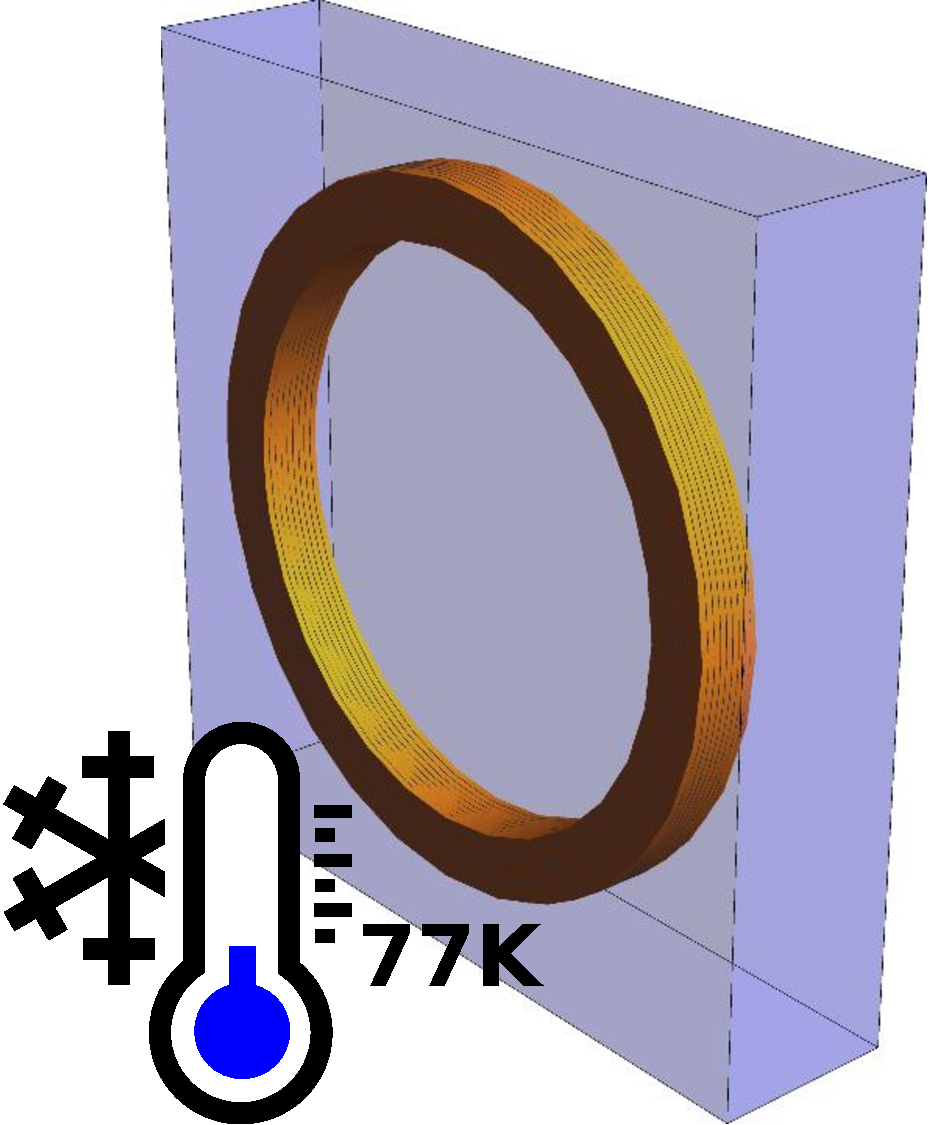
\includegraphics[height=1.5cm]{Coil1Cold.pdf}   %TODO: add "LN2" text in the image
& 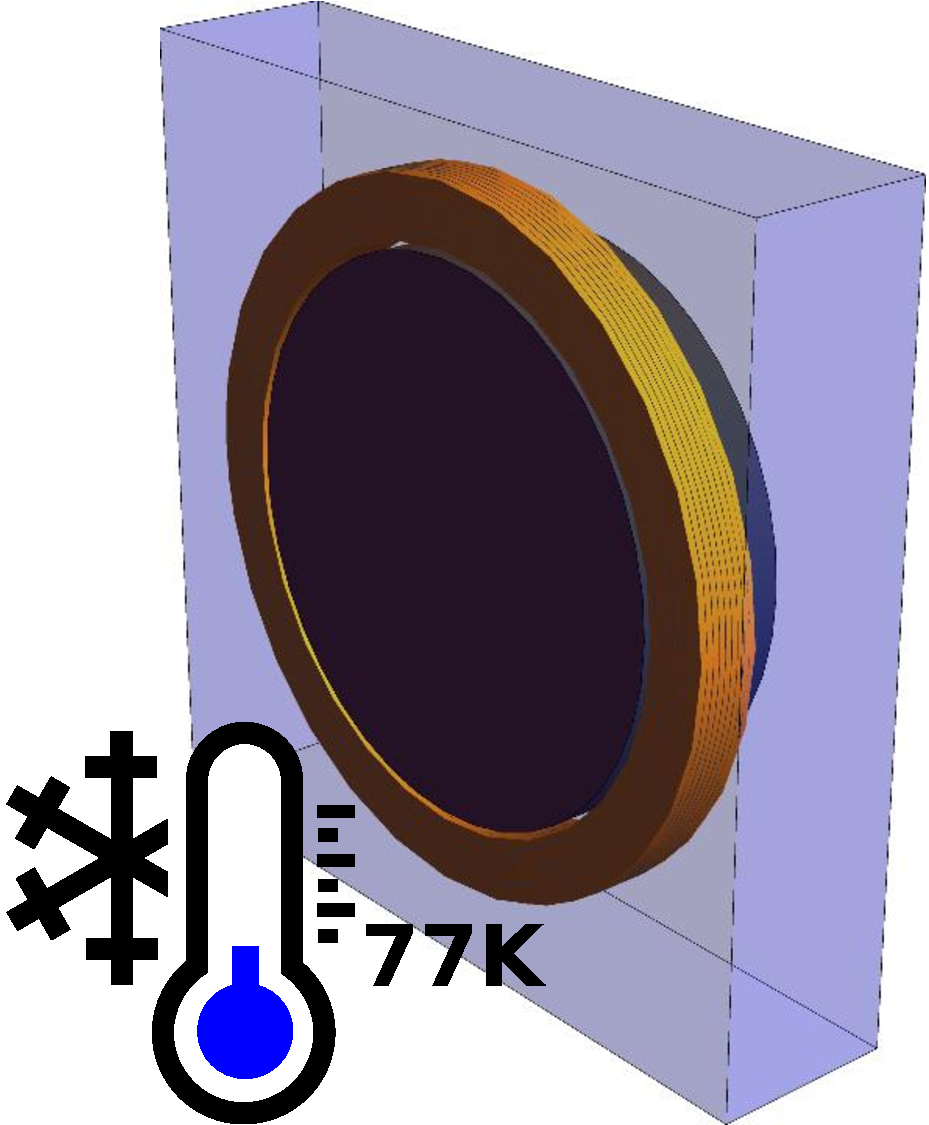
\includegraphics[height=1.5cm]{Coil2Cold.pdf} 
& 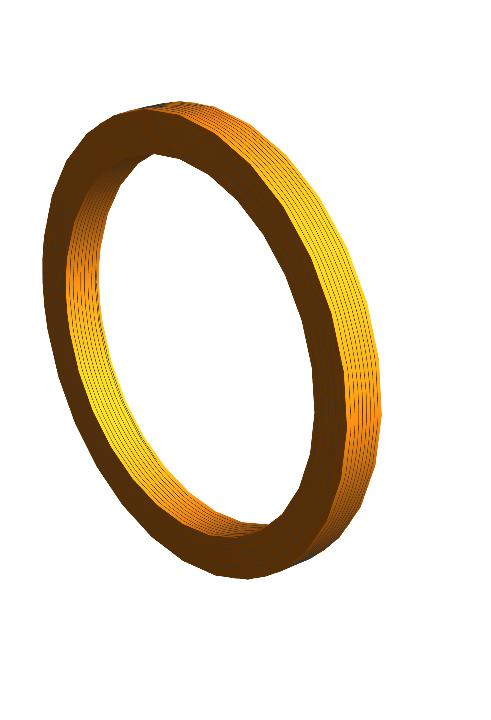
\includegraphics[height=1.5cm]{Coil3.jpg} 
& 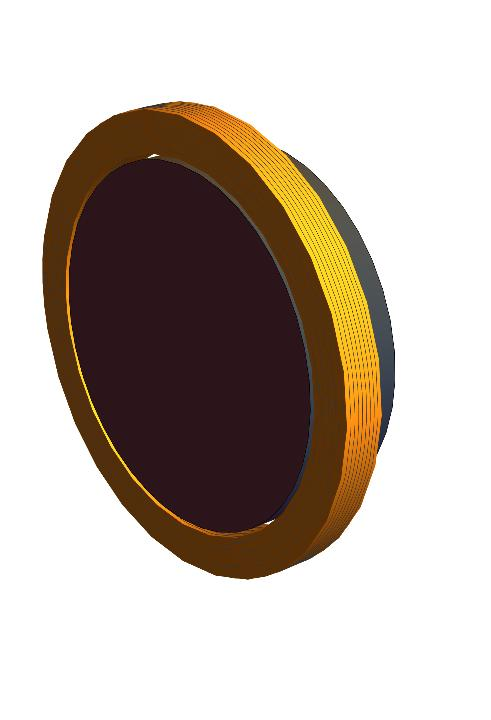
\includegraphics[height=1.5cm]{Coil4.jpg} 
& 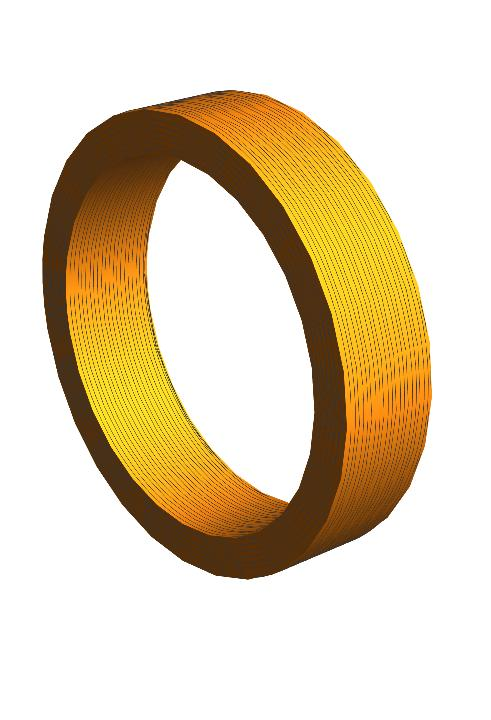
\includegraphics[height=1.5cm]{Coil5.jpg} 
& 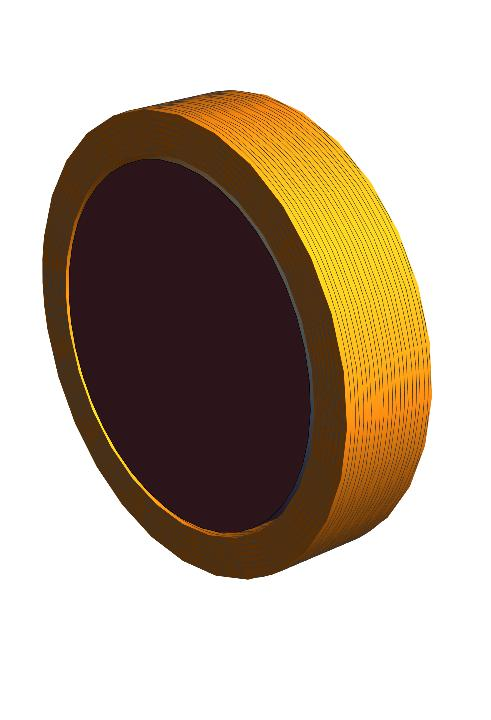
\includegraphics[height=1.5cm]{Coil6.jpg} 
\\\bottomrule
\end{tabular}}
% 
\end{table*}

%
\begin{figure}
\centering
	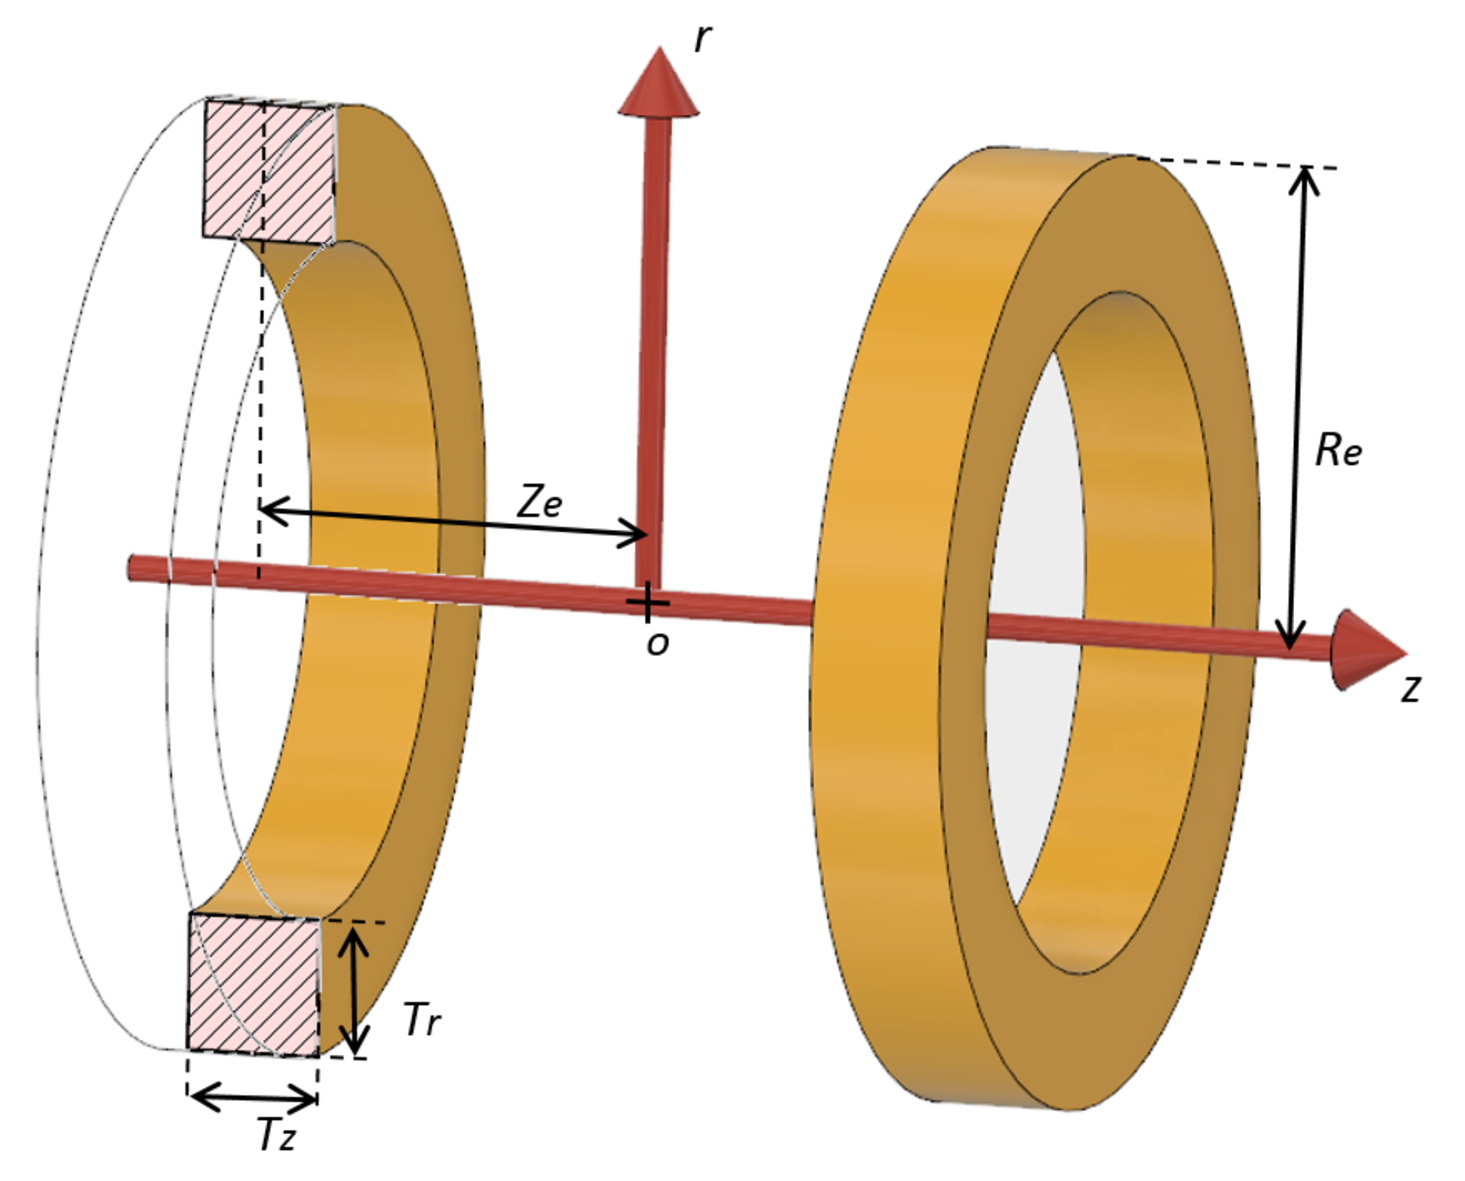
\includegraphics[width=0.5\linewidth]{3dView.eps}
	\caption{3D representation of a dual-coil collinear EM assembly.}
	\label{fig:3dView}
	\end{figure}


\begin{figure}
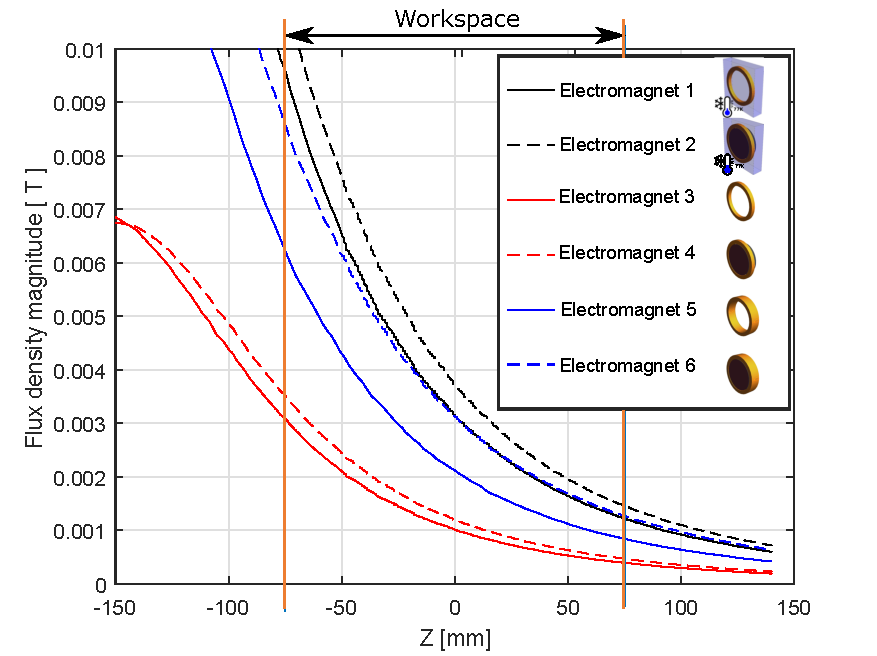
\includegraphics[width=\linewidth]{ComparisonMagnetsDesigns.pdf}
	\caption{ Maximum sustainable magnetic flux density  by different EM designs. Magnet specifications are given in Table \ref{DesignsCompare}.
	\label{fig:ComparisonMagnetsDesigns}}
\end{figure}

\begin{table}[]
\centering
\caption{Comparison between EM properties at room temperature (300K) and at LN2 temperature (77K).}
\label{CoolingComparison}
\begin{tabular}{@{}cccc@{}}
\toprule
 & 300K & 77K & Difference \\ \midrule
Copper electrical resistivity & 1.68E-8 $\Omega\cdot$m & 2.15E-9 $\Omega\cdot$m & -87\% \\ 
Coil electrical resistance & 27.3 $\Omega$ & 3.5 $\Omega$ & -87\% \\ 
Max continuous current & 1.4 A & 7.5 A & +435\% \\ 
Max cont. current density & 4.3 A/mm$^2$ & 23 A/mm$^2$ & +435\% \\ 
\bottomrule
\end{tabular}
\end{table}

\subsection{Scaling Law}

This section uses analytical equations to derive the gradient produced by two concentric electromagnets on their revolution axis (see Fig. \ref{fig:3dView}). The electromagnets have an external radius $R_e$. They have a rectangular $T_z \times T_r$ cross-section. The filling factor $F_{\textrm{Fill}} $ is assumed to be equal to 0.7. LN2 cooled magnets have an additional insulation that has a thickness $T_{\textrm{insul}}$ which reduces the internal bore diameter $D_b$.

The flux density $B_u$ produced by a single current loop can be calculated on its revolution axis using the Biot-Savart law:
%
\begin{equation}
B_{u}(R_u,Z_u)={\frac{\mu _0\cdot I_{u}}{2}}\cdot\left ( {\frac{R_{u}^2}{R_{u}^2+Z_u^2}} \right )^{\frac{3}{2}},
\label{bloop}
\end{equation}
%
where $R_u$ is the radius of the loop and $Z_u$ is the distance along the axis between the calculation point and the center of the loop.
The axial flux density created by a single finite EM is obtained by integrating this equation over the EM cross section:
%
\begin{align}
&\scalebox{.88}{$
B_e(R_e,Z_e) =
{\frac{J \mu _0   F_{\textrm{Fill}} }{2}} \int_{Z_e-T_z/2}^{Z_e+T_z/2} \int_{R_e-T_r}^{R_e} \left ( {\frac{R_{u}^2}{R_{u}^2+Z_u^2}} \right )^{\frac{3}{2}} \d R_u  \d Z_u 
$} \\
 &~~\scalebox{.7}{$=
  \frac{J \mu _0   F_{\textrm{Fill}}}{8}\left((T_z+2 Z_e) \left(\sqrt{4 R_e^2+(T_z+2 Z_e)^2}-\sqrt{4 (R_e-T_r)^2+(T_z+2 Z_e)^2}\right) \right. 
  $}  \nonumber \\
  & \qquad ~~~ \scalebox{.7}{$\left.+(T_z-2 Z_e) \left(\sqrt{4 R_e^2+(T_z-2 Z_e)^2}-\sqrt{4 (R_e-T_r)^2+(T_z-2 Z_e)^2}\right)\right)$} \nonumber
\label{Be}
\end{align}
%
where $R_e$ is the external radius of the coil, $Z_e$ is the distance along the axis between the calculation point and the center of the coil, and $J$ is the current density inside the copper wire.
 The quantity $J\cdot F_{\textrm{Fill}} $ is the current density averaged over the winding $T_z \times T_r$ cross section.
  The magnetic gradient $G_e$ is calculated by the derivative of this equation with respect to $Z_e$:
\begin{equation}
G_e=\frac{\d B_e}{\d Z_e}
\label{Ge}
\end{equation}

The total power $P_e$ dissipated inside the EM can be computed with:
%
\begin{equation}
P_e=\iiint_V F_{\textrm{Fill}}  \cdot \rho\cdot J^2 \,\d v, 
\label{Pe}
\end{equation}
%
over the volume $V$:
\begin{equation}
\scalebox{.9}{$V=\pi\ \left ( 2R_e \left ( R_e- T_{\textrm{insul}} -D_b \right ) -\left ( R_e-T_{\textrm{insul}}-D_b \right )^2\right ).$}
\label{V70cm}
\end{equation}
%
These equations were implemented in {\sc Matlab} with $T_z = T_r$. The function \texttt{fminsearch} was used to inverse this equation and find the value of $T_z$ that produces the desired gradient $G_e$ for a given $R_e$ and $Z_e$.

Fig. \ref{fig:ScalingLaw} presents simulation results obtained using equations \ref{bloop} to \ref{Pe}. Plot \emph{(a)} graphs the EM winding volume as a function of its external diameter. The blue and red curves present the $T_z$ that produces a gradient of 20 mT/m and 45 mT/m respectively. The value of $T_z$ and therefore the volume of the winding changes along these curves to produce the desired gradient strength.

Black curves have been added to locate the functioning points for a human-size system. They represent systems that have a 0.7 m bore diameter $D_b$ (similar to the bore diameters of MRI scanners). Dashed lines are plotted for an air cooled magnet while solid lines are for EM cooled with LN2.



To summarize, colored curved show systems that are able to produce a given gradient (20 mT/m for red curves and 45 mT/m for blue curves). 
 The value of $D_b$ is changing along these curves. Black curves represent systems that have $D_b$ values of 0.7 m. 
 The produced gradient strength is changing along these curves. 
  The intersections of the black and colored curves represent functioning points of systems able to produce a given gradient strength with a $D_b$ value of 0.7 m.
Plot \emph{(b)} in Fig.~\ref{fig:ScalingLaw} is similar to plot \emph{(a)} except that the results are presented in terms of power consumption. These data were obtained from the results presented in plot \emph{(a)} and calculated using eq. \ref{Pe}.

Results show that the windings of LN2 cooled systems are always smaller than air cooled windings. They also always use less power. A human-size system producing 45 mT/m would require EMs with a volume of 0.0117 m$^3$ and 0.0585 m$^3$ for LN2 and air-cooled EM respectively. Their power consumptions are respectively 17.2 kW and 8.56 kW. The use of LN2 therefore allows a reduction of 80\% of the winding volume and a decrease of 50\% of the power consumption.




\begin{figure}
	\centering
	\begin{overpic}[width=0.45\columnwidth]{ScalingLaw.eps}
	\end{overpic}
	\caption{Plot of the winding volume (a) and power consumption (b) of air-cooled (300K) and LN2-cooled (77K) EMs. 
	Red curves correspond to magnetic assemblies able to produce a gradient strength of 20 mT/m at the system center.
	 Blue curves correspond to magnetic assemblies  able to produce a gradient strength of 45 mT/m at the system center.}
	\label{fig:ScalingLaw}
\end{figure}



\section{Inverse Magnetics}\label{sec:invMagnetics}
This section analyzes 3D manipulation of a single robot having a magnetization $\mathbf{m}$. The magnetic manipulator is composed of six EM controlled by independent current sources. The total magnetic field is the sum of the field produced by each coil.
 This section calculates the coil current values to produce the desired force and torque on the robot or the desired force and magnetic field orientation.

\subsection{Forward problem} \label{Forward}
%To simplify the analysis, the forward problem will first be solved, i.e. from the current values, the force and flux density will be calculated.
To simplify analysis, we first solve the \emph{forward problem} which computes the force and flux density or force and torque using the coil currents. 

The system has six EMs, numerated from 1 to 6.
The magnetic flux density $B_{k(\mathbf{P})}$ produced by EM number $k$ at location $\mathbf{P}$ can be calculated using eq. \ref{FieldEq} where $I_k$ is the current in the magnet and $\mathbf{B}_{k(\mathbf{P})}$ is a function that depends on the geometry of the system and the position of the magnet. The function $\mathbf{B}_{k(\mathbf{P})}$ is computed assuming that the coils are equivalent to current loops. The flux density produced by a current loop is calculated using the semi-analytical equations presented in \cite{simpson2001simple}.
%
\begin{equation}
\mathbf{B}_{k(\mathbf{P})}=\begin{bmatrix}
B_{kx}
\\
B_{ky} 
\\ 
B_{kz}
\end{bmatrix}=\mathbf{\widetilde{B}}_{k(\mathbf{P})}\cdot I_k=
\begin{bmatrix}
{\widetilde{B}}_{kx(\mathbf{P})}
\\
{\widetilde{B}}_{ky(\mathbf{P})}
\\ 
{\widetilde{B}}_{kz(\mathbf{P})}

\end{bmatrix}\cdot I_k
\label{FieldEq}
\end{equation}
%
The flux density produced by the complete system can be computed by summing the field produced by each magnet (see eq.~\ref{FieldTot}) where $\mathbf{I}$ is a vector containing the current of each coil.
%
\begin{dmath}
\mathbf{B}_{(\mathbf{P})}= \scalebox{.8}{$\left(\mathbf{\widetilde{B}}_{1(\mathbf{P})}+\mathbf{\widetilde{B}}_{2(\mathbf{P})}+\mathbf{\widetilde{B}}_{3(\mathbf{P})}+\mathbf{\widetilde{B}}_{4(\mathbf{P})}+\mathbf{\widetilde{B}}_{5(\mathbf{P})}+\mathbf{\widetilde{B}}_{6(\mathbf{P})}\right )\mathbf{I} $}
\label{FieldTot}
\end{dmath}
%
It is now necessary to define three new vectors:
%
\begin{align}
\mathbf{\widetilde{B}}_{x(\mathbf{P})}&= \scalebox{.85}{$\setlength\arraycolsep{2pt} \begin{bmatrix}
\widetilde{B}_{1x(\mathbf{P})} & \widetilde{B}_{2x(\mathbf{P})} & \widetilde{B}_{3x(\mathbf{P})} & \widetilde{B}_{4x(\mathbf{P})} & \widetilde{B}_{5x(\mathbf{P})} & \widetilde{B}_{6x(\mathbf{P})}
\end{bmatrix}$}
\label{Gx} \\
%
\mathbf{\widetilde{B}}_{y(\mathbf{P})}&= \scalebox{.85}{$\setlength\arraycolsep{2pt}
\begin{bmatrix}
\widetilde{B}_{1y(\mathbf{P})} & \widetilde{B}_{2y(\mathbf{P})} & \widetilde{B}_{3y(\mathbf{P})} & \widetilde{B}_{4y(\mathbf{P})} & \widetilde{B}_{5y(\mathbf{P})} & \widetilde{B}_{6y(\mathbf{P})}
\end{bmatrix}$}
\label{Gy} \\
%
\mathbf{\widetilde{B}}_{z(\mathbf{P})}&= \scalebox{.85}{$\setlength\arraycolsep{2pt} \begin{bmatrix}
\widetilde{B}_{1z(\mathbf{P})} & \widetilde{B}_{2z(\mathbf{P})} & \widetilde{B}_{3z(\mathbf{P})} & \widetilde{B}_{4z(\mathbf{P})} & \widetilde{B}_{5z(\mathbf{P})} & \widetilde{B}_{6z(\mathbf{P})}
\end{bmatrix}$}
\label{Gz}
\end{align}
%
Equation \ref{FieldTot} can be re-written as follows:
\begin{equation}
\mathbf{B}_{(\mathbf{P})}=\begin{bmatrix}
\mathbf{\widetilde{B}}_{x(\mathbf{P})}
\\
\mathbf{\widetilde{B}}_{y(\mathbf{P})}
\\ 
\mathbf{\widetilde{B}}_{z(\mathbf{P})}
\end{bmatrix}\cdot\mathbf{I}
\end{equation}
%
The force $\mathbf{F}$ is calculated with:
%
\begin{equation}
\mathbf{F}=\begin{bmatrix}
F_{x(\mathbf{P})}
\\ 
F_{y(\mathbf{P})}
\\ 
F_{z(\mathbf{P})}
\end{bmatrix}
=\mathbf{\nabla}\cdot\left ( \mathbf{m}\cdot\mathbf{B}_{(\mathbf{P})} \right ),
\label{Force}
\end{equation}
%
which can be re-written as:
%
\begin{equation}
\boldsymbol{F}=\begin{bmatrix}
m_x\cdot\frac{{\partial {\mathbf{\widetilde{B}}}_{x(\mathbf{P})}}}{\partial x}+m_y\cdot\frac{{\partial {\mathbf{\widetilde{B}}}_{y(\mathbf{P})}}}{\partial x}+m_z\cdot\frac{{\partial {\mathbf{\widetilde{B}}}_{z(\mathbf{P})}}}{\partial x}
\\ 
m_x\cdot\frac{{\partial {\mathbf{\widetilde{B}}}_{x(\mathbf{P})}}}{\partial y}+m_y\cdot\frac{{\partial {\mathbf{\widetilde{B}}}_{y(\mathbf{P})}}}{\partial y}+m_z\cdot\frac{{\partial {\mathbf{\widetilde{B}}}_{z(\mathbf{P})}}}{\partial y}
\\ 
m_x\cdot\frac{{\partial {\mathbf{\widetilde{B}}}_{x(\mathbf{P})}}}{\partial z}+m_y\cdot\frac{{\partial {\mathbf{\widetilde{B}}}_{y(\mathbf{P})}}}{\partial z}+m_z\cdot\frac{{\partial {\mathbf{\widetilde{B}}}_{z(\mathbf{P})}}}{\partial z}
\end{bmatrix}\cdot\mathbf{I}
\end{equation}
%
The torque $\mathbf{T}$ is calculated with:
%
\begin{equation}
\mathbf{T}=\begin{bmatrix}
T_{x(\mathbf{P})}
\\ 
T_{y(\mathbf{P})}
\\ 
T_{z(\mathbf{P})}
\end{bmatrix}
=\mathbf{m}\times\mathbf{B}
\label{Torque}
\end{equation}
%
which can be re-written as:
%
\begin{equation}
\mathbf{T}=\begin{bmatrix}
m_y\cdot \mathbf{\widetilde{B}}_{z(\mathbf{P})}-m_z\cdot \mathbf{\widetilde{B}}_{y(\mathbf{P})}
\\
m_z\cdot \mathbf{\widetilde{B}}_{x(\mathbf{P})}-m_x\cdot \mathbf{\widetilde{B}}_{z(\mathbf{P})}
\\ 
m_x\cdot \mathbf{\widetilde{B}}_{y(\mathbf{P})}-m_y\cdot \mathbf{\widetilde{B}}_{x(\mathbf{P})}
\end{bmatrix}\cdot \mathbf{I}
\label{TorqueMatrix}
\end{equation}

\subsection{Inverse problem}
Two inverse methods are studied. The first one aims at controlling the flux density and the force applied on the robot using the actuation matrix $\mathbf{A_0}$:
%
\begin{equation}
\mathbf{A_0}=\begin{bmatrix}
\mathbf{\widetilde{B}}_{x(\mathbf{P})}
\\
\mathbf{\widetilde{B}}_{y(\mathbf{P})}
\\ 
\mathbf{\widetilde{B}}_{z(\mathbf{P})}
\\ 
m_x\cdot\frac{{\partial {\mathbf{\widetilde{B}}}_{x(\mathbf{P})}}}{\partial x}+m_y\cdot\frac{{\partial {\mathbf{\widetilde{B}}}_{y(\mathbf{P})}}}{\partial x}+m_z\cdot\frac{{\partial {\mathbf{\widetilde{B}}}_{z(\mathbf{P})}}}{\partial x}
\\ 
m_x\cdot\frac{{\partial {\mathbf{\widetilde{B}}}_{x(\mathbf{P})}}}{\partial y}+m_y\cdot\frac{{\partial {\mathbf{\widetilde{B}}}_{y(\mathbf{P})}}}{\partial y}+m_z\cdot\frac{{\partial {\mathbf{\widetilde{B}}}_{z(\mathbf{P})}}}{\partial y}
\\ 
m_x\cdot\frac{{\partial {\mathbf{\widetilde{B}}}_{x(\mathbf{P})}}}{\partial z}+m_y\cdot\frac{{\partial {\mathbf{\widetilde{B}}}_{y(\mathbf{P})}}}{\partial z}+m_z\cdot\frac{{\partial {\mathbf{\widetilde{B}}}_{z(\mathbf{P})}}}{\partial z}
\end{bmatrix}
\end{equation}
%
The force and flux density are equal to:
\begin{equation}
\label{FullEq}
\begin{bmatrix}
\mathbf{B}
\\ 
\mathbf{F}
\end{bmatrix}=\mathbf{A_0}\cdot\mathbf{I}
\end{equation}
$\mathbf{A_0}$ is a square matrix and can be inverted provided that it is not singular. The current $\mathbf{I}$ is calculated with:
%
\begin{equation}
\mathbf{I}=\mathbf{A_0}^{-1}\cdot\begin{bmatrix}
\mathbf{B}
\\ 
\mathbf{F}
\end{bmatrix}
\end{equation}
%
The second method controls the force and torque applied on the robot using the actuation matrix $\mathbf{A_1}$
%
\begin{equation}
\mathbf{A_1}=\begin{bmatrix}
m_y\cdot \mathbf{\widetilde{B}}_{z(\mathbf{P})}-m_z\cdot \mathbf{\widetilde{B}}_{y(\mathbf{P})}
\\
m_z\cdot \mathbf{\widetilde{B}}_{x(\mathbf{P})}-m_x\cdot \mathbf{\widetilde{B}}_{z(\mathbf{P})}
\\ 
m_x\cdot \mathbf{\widetilde{B}}_{y(\mathbf{P})}-m_y\cdot \mathbf{\widetilde{B}}_{x(\mathbf{P})}
\\
m_x\cdot\frac{{\partial {\mathbf{\widetilde{B}}}_{x(\mathbf{P})}}}{\partial x}+m_y\cdot\frac{{\partial {\mathbf{\widetilde{B}}}_{y(\mathbf{P})}}}{\partial x}+m_z\cdot\frac{{\partial {\mathbf{\widetilde{B}}}_{z(\mathbf{P})}}}{\partial x}
\\ 
m_x\cdot\frac{{\partial {\mathbf{\widetilde{B}}}_{x(\mathbf{P})}}}{\partial y}+m_y\cdot\frac{{\partial {\mathbf{\widetilde{B}}}_{y(\mathbf{P})}}}{\partial y}+m_z\cdot\frac{{\partial {\mathbf{\widetilde{B}}}_{z(\mathbf{P})}}}{\partial y}
\\ 
m_x\cdot\frac{{\partial {\mathbf{\widetilde{B}}}_{x(\mathbf{P})}}}{\partial z}+m_y\cdot\frac{{\partial {\mathbf{\widetilde{B}}}_{y(\mathbf{P})}}}{\partial z}+m_z\cdot\frac{{\partial {\mathbf{\widetilde{B}}}_{z(\mathbf{P})}}}{\partial z}
\end{bmatrix}
\label{A1}
\end{equation}

The torque and force are equal to:

\begin{equation}
\label{FullEq2}
\begin{bmatrix}
\mathbf{T}
\\ 
\mathbf{F}
\end{bmatrix}=\mathbf{A_1}\cdot\mathbf{I}
\end{equation}
$\mathbf{A_1}$ is a square matrix and can be inverted provided that it is not singular. The current $\mathbf{I}$ is calculated with:
\begin{equation}
\mathbf{I}=\mathbf{A_1}^{-1}\cdot\begin{bmatrix}
\mathbf{T}
\\ 
\mathbf{F}
\end{bmatrix}
\label{FullEq3}
\end{equation}


\section{Trajectory control}\label{sec:TrajectoryControl}


Equation \ref{FullEq} shows that $\mathbf{F}$ is decoupled from $\mathbf{B}$ and $\mathbf{T}$. The control of $\mathbf{B}$ enables the control of the orientation of the robot. The robot can be assumed to be oriented along the magnetic field direction, as in~\cite{kummer2010octomag}. The magnitude of the flux density $|\mathbf{B}|$ is set to a constant value and the individual components are calculated to obtain the desired field orientation. Another alternative is to use eq. \ref{FullEq3} to control the torque directly.

The trajectory is controlled using the controller presented in Fig.~\ref{fig:Controller}(b). It uses a nested control structure. 
The inner PID control loop regulates velocity, which is limited by a saturation function to avoid excessive speeds and instabilities. 
The outer loop generates a velocity setpoint.\par

The trajectory is defined by the user as a set of of viapoints and the corresponding desired velocities $V_t$. The outer loop first searches for the point of the trajectory that is the closest to the robot position and determines $V_t$. An additional velocity component $V_s$ is added to this value to steer the robot toward the trajectory centerline.\par
  
When the calculated current is above the maximum value ($I_{\textrm{max}}$ is the maximum current the power supplies can generate) the vector $\mathbf{I}$ is scaled down so that the largest element of $\mathbf{I}$ is equal to $I_{\textrm{max}}$. 
This reduces the force and flux density values applied on the robot, but has the advantage of keeping the correct field and force orientation. 



\section{Singularities analysis for a 3-DOF robot} \label{sec:singularities}
%\begin{figure}
	%\begin{overpic}[width=\linewidth]{Condition.eps}
	%\put(32,86){\includegraphics[width=0.4cm]{TinyMag0.pdf}}
	%\put(83,86){\includegraphics[width=0.4cm]{TinyMag90.pdf}}
	%\put(32,41){\includegraphics[width=0.4cm]{TinyMagn45.pdf}}
	%\put(83,41){\includegraphics[width=0.4cm]{TinyMag45.pdf}}
	%\end{overpic}
	%\caption{Condition number of $\mathbf{A}$ at four robot angle $\theta$ values.}
	%\label{Condition}	
%\end{figure}

\begin{figure}
	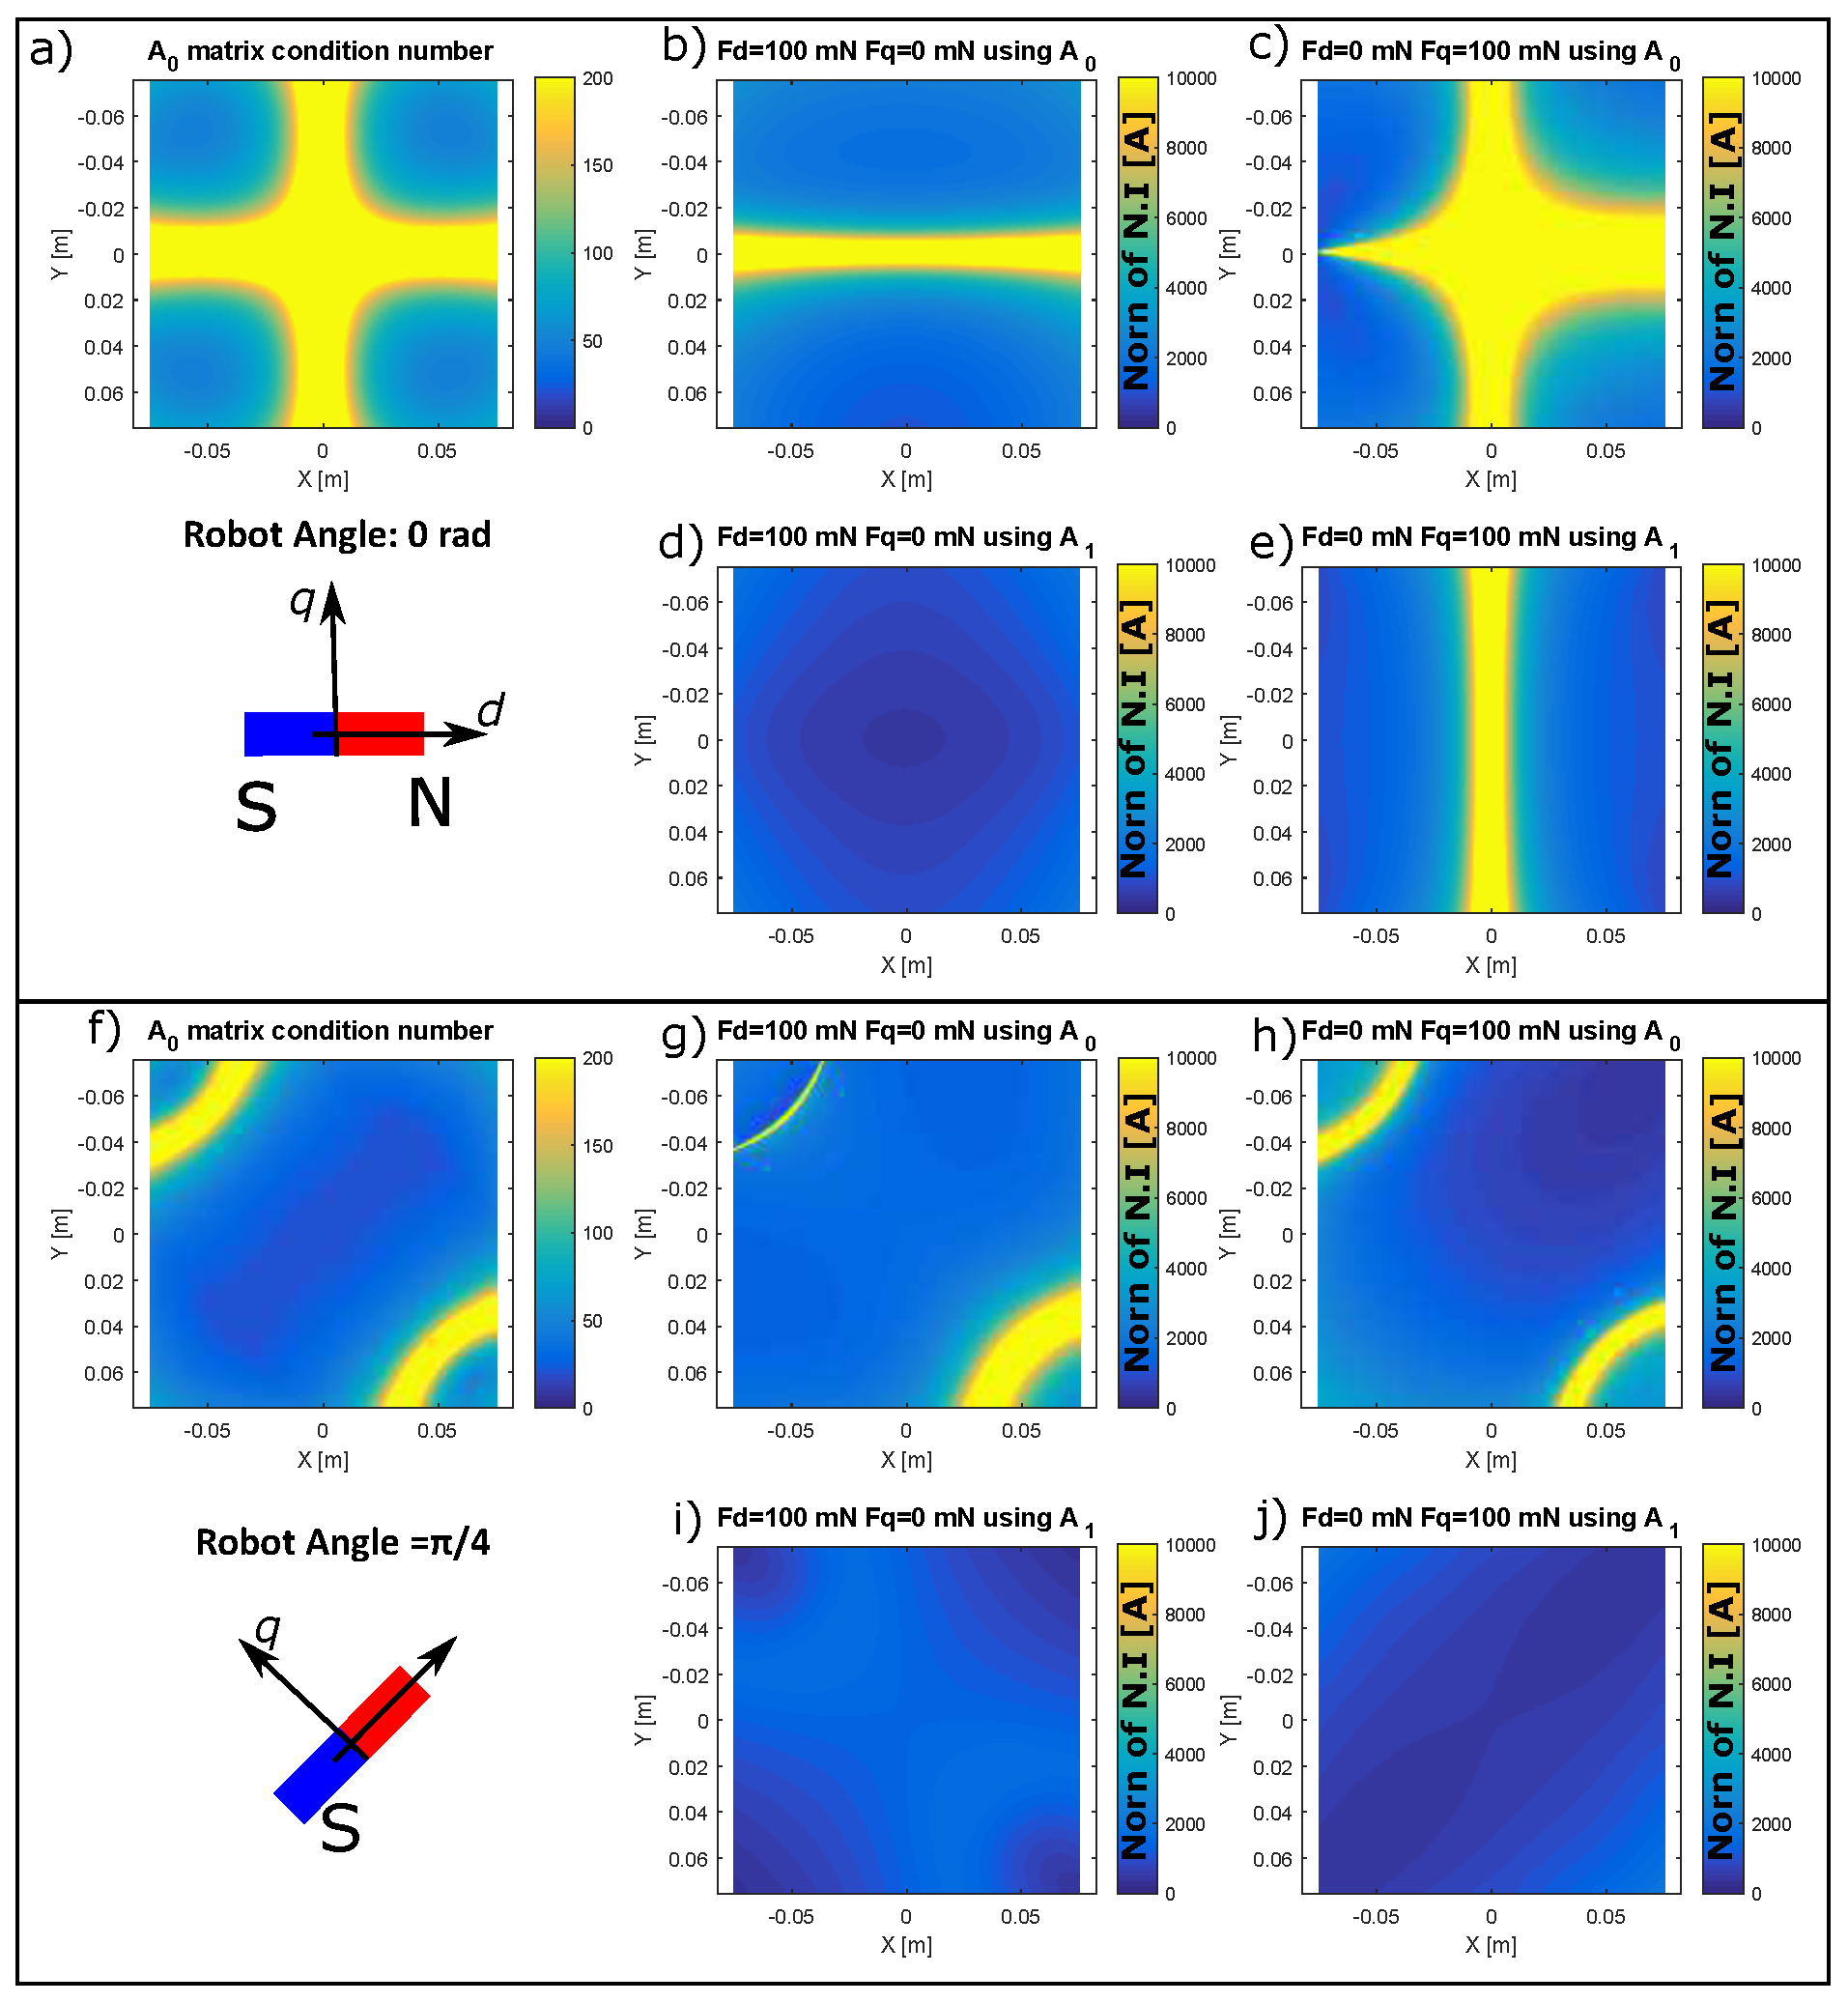
\includegraphics[width=\linewidth]{Conditioning3.eps}
	\caption{Map of the conditioning of the actuation matrix $\mathbf{A_0}$ for (a) $\theta=0$ and (f) $\theta=\pi/4$. 
	Map of the norm of the total current needed to produce a force of 100 mN along the $d$ axis (plots b, d, g and i) and along the $q$ axis (plots c, e, h and j). 
	Plots b, c, d and e are plotted for $\theta=0$ and plots g, h, i and j are plotted for $\theta=\pi/4$.
	Plots b, c, g and h were calculated using $\mathbf{A_0}$ and plots d, e, i and j were calculated using $\mathbf{A_1}$. }
	\label{condition}
\end{figure}


As explained in \S\ref{sec:TrajectoryControl}, the orientation of the robot can be controlled using two different methods. 
 The first one uses actuation matrix $\mathbf{A_0}$ and allows applying a desired flux density vector $\mathbf{B}$ and a force $\mathbf{F}$ to the robot. 
 The second uses actuation matrix $\mathbf{A_1}$ and allows applying a desired torque $\mathbf{T}$ and a force $\mathbf{F}$ to the robot.

When expressed in the manipulator coordinate system ($x,y,z$), $\mathbf{A_1}$ is square. However, the robot is symmetric around its revolution axis $d$ and therefore no torque can be applied on the $d$ axis. Defining a new coordinate system ($d,q,w$) allows removing one dimension from $\mathbf{A_1}$ (i.e. $\mathbf{A_1}$ has a size 5$\times$6 when expressed in the ($d,q,w$) coordinate system). The system is therefore underdetermined and the least square solution is calculated using eq. \ref{LS}.
 
\begin{equation}
\label{LS}
\mathbf{I}=\mathbf{A_1}^{T}\left ( \mathbf{A_1} \cdot \mathbf{A_1}^{T} \right )^{-1}\cdot \begin{bmatrix}
\mathbf{T}
\\ 
\mathbf{F}
\end{bmatrix}
\end{equation}

The actuation matrices $\mathbf{A_0}$ and $\mathbf{A_1}$ are functions of the magnetic manipulator geometry and the robot pose. 

The effect of singularities was studied for a 2D--3DOF control. The magnet is horizontally placed on a flat surface corresponding to the $x$-$y$ plane. The robot is able to move along $x$ and $y$ and rotate around the $z$-axis.

A 4$\times$4 $\mathbf{A_0}$ and a 4$\times$3 $\mathbf{A_1}$ actuation matrices can be calculated for each robot position and angle. The map of the conditioning of the $\mathbf{A_0}$ matrix is shown in Fig.~\ref{condition}(a) and (f). On this figure is also presented the norm of the total current $N \cdot \mathbf{I}$ required to produce a force of 100 mN along the $d$-axis (central-column) and $q$-axis (right-column). Plots for $\theta=0$ and $\theta=\pi/4$ are presented. Results for other angles are shown in the attached video.  

For $\theta=0$, $\mathbf{A_0}$ has two singularity lines on the $x$ and $y$ axis. For $\theta=\pi/4$ singularities take a rounded shape and are located on two opposite angles of the workspace. No solution is available when the matrix is singular. The singularities are situated on infinitely thin lines, but the system is ill-conditioned near the singularity lines. A large condition number produces a large magnitude for the $\mathbf{I}$ vector. The capabilities of the power supplies limit the maximum current and when the condition number becomes too large, the current saturates. This saturation decreases control authority over the robot in these regions.\par

The norm of the total current $N \cdot \mathbf{I}$ needed to produce a force of 100 mN along the $d$ and $q$ axis was calculated as a function of the robot position and angle. Plots b, c, e and f of Fig.~\ref{condition} present these results. When using the $\mathbf{A_0}$ matrix, there are areas where the current becomes larger than 10,000~A close to the singularities when the force is generated along the $d$ axis as well as when the force is generated along the $q$ axis. When using $\mathbf{A_1}$, these large current densities are present only when a force is generated along the $q$ axis. When the force is produced along the $d$ axis, the current always stays within relatively small values. This observation is valid for any robot orientation.

\section{Experimental Results}
\label{Experiment}
\begin{figure}
\includegraphics[width=\linewidth]{EllipseTrajectory.eps}
\vspace{-2em}
	\caption{Plot of the trajectory of the robot obtained experimentally. For this dataset, the robot completed the path ten times. The robot and the workspace are shown at right.}
	\label{Path}	
\end{figure}

\begin{figure}
	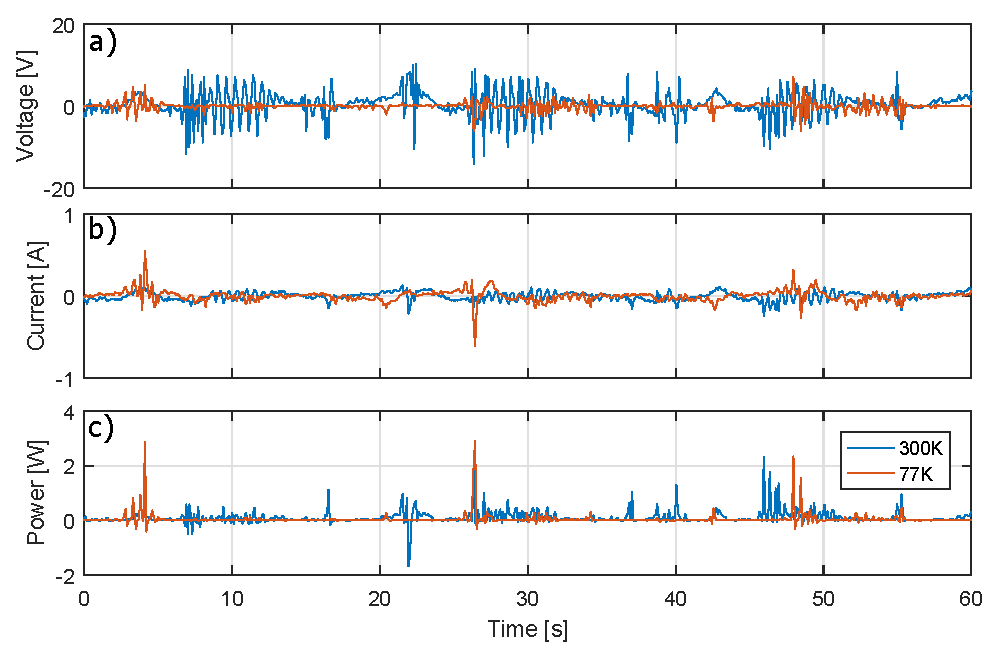
\includegraphics[width=\linewidth]{Waveform.eps}
	\caption{Voltage, current, and power used during robot navigation. The curves show 60 seconds of data, which correspond to the robot completing the trajectory in Fig.~\ref{Path} three times.}
	\label{waveform}
\end{figure}

The control of the velocity and orientation of a NdFeB permanent magnet in a 2D plane described in \S\ref{sec:TrajectoryControl} was implemented and tested using the $\mathbf{A_1}$ actuation matrix. As shown in \S\ref{sec:singularities} it is preferable to apply the force along the magnetization axis of the robot ($d$-axis). The program was therefore configured to orient the robot magnetization in the same direction as the applied force. This allows minimizing the value of the force applied along the $q$ axis and therefore improve stability by avoiding current saturations.
% As shown in \S\ref{sec:singularities} 
The permanent magnet was cylindrical, with a diameter of 2.5 mm and a length of 10 mm. 
It was encapsulated in a black shrink tube to facilitate computer vision tracking. 
The magnet was then attached horizontally on a Styrofoam disk having a diameter of 18 mm and a thickness of 6 mm. 
Pictures of the robot are shown in Fig.~\ref{Path}. 

A robot navigating inside fluid-filled cavities of the human body may be designed to have neutral buoyancy to reduce the amount of force needed. 
To simulate neutral buoyancy in this 2D control experiment, the magnet-Styrofoam assembly floated at the surface of a water-filled tank. The magnet was able to move freely in the $x$ and $y$ directions as well as rotate around the $z$ axis.\par
The method from \S\ref{sec:TrajectoryControl} was used with the $\mathbf{A_1}$ actuation matrix from \eqref{A1}.
 The trajectory was an ellipse having a major axis of 63 mm and a minor axis of 40 mm.

Test were performed with and without LN2 cooling. The trajectory obtained experimentally without LN2 is presented in Fig.~\ref{Path}. For these plots, the robot followed the trajectory ten times. Trajectories obtained with LN2 cooling are similar. The robot was stable during the navigation, but small deviation from the centerline were observed at several locations. 

The current and voltage applied on the $-x$ EM was recorded during one minute for both cooling methods. The instantaneous power was calculated from these data and the results are presented in Fig. \ref{waveform}. The average power used for the air cooled case is equal to 0.218 W whereas it is only equal to 0.037 W when magnets are cooled with LN2.  This decrease of average power consumption is enabled by the decrease of copper electrical resistivity when cooled at 77K and produces a decrease of the applied voltage as shown in  Fig.~\ref{waveform}(a).  The parameters of the controller were not changed between the tests, however, the peak power is increased when LN2 is added. This behavior could be explained by an increase of the current regulation dynamics performed by the power supply when the electrical resistance of the EM is decreased by the cooling. 

The power used was low because the floating robot required little force.
%The values of power obtained are low due to the fact that the force that needs to be applied on a floating robot to move it is very small. 
Applications that navigate against flow or perform surgery require larger forces and correspondingly more power.


 
% 
%The conclusion looks like a summary. It shouldn�t. You can focus on if
%your main hypotheses of the paper could be supported by the experiment
%etc., and other derivatives of the hypotheses.
%%%%%%%%%%%%%%%%%%%%%%%%%%%%%%%%%%%%%%%%%%%%%%%%%%%%%
\section{Conclusion and Future Works}
%%%%%%%%%%%%%%%%%%%%%%%%%%%%%%%%%%%%%%%%%%%%%%%%%%%%%
This paper presented a magnetic manipulator using EM cooled with LN2. 
Liquid nitrogen cooling allows increasing the current circulating inside an EM up to 435\%. 
This cooling enables reducing the size of the EM to produce a given magnetic field. 
The required electromagnets to achieve a given flux density are cheaper to build, and the complete system is more compact. 
%Air-core LN2-cooled EM can, unlike iron-core magnets, have an open bore. 
%This feature is necessary for medical applications where the magnetic system needs to be open on at least two opposite ends to accommodate the patient.
\par
%
A desktop-size prototype was built and tested. 
The robot, a cylindrical permanent magnet, was manipulated on a 2D plane. 
Three DOF were controlled: the orientation and the $x$ and $y$ positions.\par
%
The system was not designed to produce a uniform magnetic field. 
Instead, inverse magnetic calculations account for field non-uniformities.
The current inside each coil is computed to generate the desired force on the robot and produce the desired field orientation. 
 %The calculations include a function that computes the field produced by each coil in space. 
 %The coils are assumed to be equivalent to circular current loops.
 \par
 %
The system's matrix conditioning was analyzed. 
 The matrix is sometimes ill-conditioned, depending on the position and orientation of the robot. 
  Issues with ill conditioning can be avoided by controlling the torque directly and avoiding the production of forces along the axis perpendicular to the robot magnetization.
  \par
  %
More control inputs can be added to improve the controllability of the robot. 
A possibility is to use additional EM, as in \cite{kummer2010octomag} where eight EMs were used to control a five DOF robot, but using additional EMs makes the system more complicated and expensive to build.
 \par
 %
Future study will focus on the addition of a high-frequency component to the magnetic field to increase the controllability of the robot. 
  A permanent magnet could be encapsulated in a conductive shell such as copper. 
  If the robot is electrically conductive, the AC field would induce currents in it, and generate an additional torque as in an induction electric motor. 
  This AC magnetic field could also be used to control resonating magnetic actuators as in \cite{vollmers2008wireless}. 
  Finally, the controller could include a temperature management feature that calculates the heat dissipated in the windings and avoids overheating by preventively reducing power.
  %Mechanically resonating millirobots were successfully tested \cite{vollmers2008wireless,frutiger2008magmites}. 
%


\chapter[Exploiting Non-Slip Wall Contacts  to Position Two Particles Using The Same Control Input]{Exploiting Non-Slip Wall Contacts  to Position Two Particles Using The Same Control Input}\label{chap-wallFriction}



This chapter is based on a journal submission with  Shiva Shahrokhi, Jingang Shi,  Benedict Isichei, and Aaron T. Becker.
My contribution was focused on ??????????.
This work was supported by the National Science Foundation under Grant No.\ \href{http://nsf.gov/awardsearch/showAward?AWD_ID=1553063}{ [IIS-1553063]} and \href{http://nsf.gov/awardsearch/showAward?AWD_ID=1619278}{[IIS-1619278]}.


Steered particles offer a method for targeted therapy, interventions, and drug delivery in regions inaccessible by large robots.
Magnetic actuation has the benefits of requiring no tethers, being able to operate from a distance, and in some cases allows imaging for feedback (e.g. MRI).
 This paper investigates particle control with uniform magnetic gradients (the same force is applied everywhere in the workspace).
Given three orthogonal magnetic fields, steering one particle in 3D is trivial. 
Adding additional particles to steer makes the system underactuated because there are more states than control inputs. 
However, the walls of in vivo and artificial environments often have surface roughness such that the particles do not move unless actuation pulls them away from the wall.
In previous work, we showed that the individual 2D position of two particles is controllable in a square workspace with non-slip wall contact \cite{shahrokhi2017algorithms}.
Because in vivo environments are usually not square, this paper extends the previous work to all convex workspaces and to 3D positioning. 
This paper also implements the algorithms using a hardware setup inspired by the gastrointestinal tract.


%%%%%%%%%%%%%%%
\section{Introduction}\label{sec:Intro}
Particle swarms propelled by a uniform field, where each particle  receives the same control input, are common in applied mathematics, biology, and computer graphics \cite{Peyer2013,Shirai2005,Chiang2011}.


The small size of these robots makes it difficult to perform onboard computation.  Instead, these robots are often controlled by a broadcast signal. 
 The tiny robots themselves are often just rigid bodies, and it may be more accurate to define the robot as the \emph{system} that consists of particles, a uniform control field, and sensing.
Such systems are severely underactuated, having 2 degrees of freedom in the shared planar control input, but $2n$ degrees of freedom for the $n$-particle swarm.
 Techniques are needed that can handle this underactuation. 

 Positioning is a foundational capability for a robotic system, e.g. placement of brachytherapy seeds. 
 In previous work, we showed that the 2D position of each particle in such a swarm is controllable if the workspace contains a single obstacle the size of one particle \cite{AaronManipulation2013}.
 However, requiring a single, small, rigid obstacle suspended in the middle of the workspace is often an unreasonable constraint, especially in 3D.
This paper relaxes that constraint, and provides position control algorithms that only require non-slip wall contacts.
We assume that particles in contact with the boundaries have zero velocity if the uniform control input pushes the particle into the wall.



\begin{figure}
\centering
\vspace{1.5em}
%\begin{overpic}[width=\columnwidth]{firstImage.jpg}\end{overpic}
\begin{overpic}[width=0.45\columnwidth]{firstpicLeft.pdf}\put(28,-10){workspace}\end{overpic}
\begin{overpic}[width=0.45\columnwidth]{magneticsetup.pdf}\put(22,-8){magnetic setup}\end{overpic}
\vspace{1em}
\caption{\label{fig:IntroPic}
Workspace and magnetic setup for an experiment to position particles that receive the same control inputs, but cannot move while a control input pushes them into a boundary.
} \vspace{-1em}
\end{figure}
%\todo{add the picture of magnetic setup}


The paper is arranged as follows. 
After a review of recent related work in Sec.  \ref{sec:RelatedWork},
 %Sec. \ref{subsec:FluidInTank} provides analytical position control results of stable configurations in two canonical workspaces with frictionless walls.  These results are limited in the set of shapes that can be generated.  To extend the range of possible shapes,
  Sec.  \ref{sec:theory} introduces a  model for boundary interaction and two shortest path results for representative workspaces.   
We provide an algorithm to arbitrarily position two particles in Sec.  \ref{sec:PostionControl2Robots}.
Section  \ref{sec:simulation} describes implementations of the algorithms in simulation and  Sec.  \ref{sec:expResults} describes hardware experiments, as shown in Fig.~\ref{fig:IntroPic}. 
 We end with directions for future research in Sec.  \ref{sec:conclusion}.

This paper is an elaboration of preliminary work in a conference paper \cite{shahrokhi2017algorithms} which considered only square workspaces. This work extends the analysis to convex workspaces and 3D positioning. This paper also implements the algorithms using a hardware setup inspired by the anatomy of the gastrointestinal tract.



%%%%%%%%%%%%%%%%%%%%%%%%%%%%%%%%%%%%%%%%%%%%%%%%%%%%%%%%%%%
\section{Related Work}\label{sec:RelatedWork}
%%%%%%%%%%%%%%%%%%%%%%%%%%%%%%%%%%%%%%%%%%%%%%%%%%%%%%%%%%%

Controlling the \emph{shape}, or relative positions, of a swarm of robots is a key ability for a range of applications.  Correspondingly, it has been studied from a control-theoretic perspective in  both centralized and decentralized approaches. For examples of each, see the centralized virtual leaders in \cite{egerstedt2001formation}, and the  gradient-based decentralized controllers  using control-Lyapunov functions in~\cite{hsieh2008decentralized}. However, these approaches assume a level of intelligence and autonomy in individual robots that exceeds the capabilities of many systems, including current micro- and nano-robots.  Current micro- and nano-robots, such as those in~\cite{Chowdhury2015,martel2015magnetotactic,Xiaohui2015magnetiteMicroswimmers} lack onboard computation.

This paper focuses on centralized techniques that apply the same control input to both particles. 
Precision control requires breaking the symmetry caused by the uniform input.  
Symmetry can be broken using particles that respond differently to the uniform control signal, either through agent-agent reactions \cite{bertozzi2015ring}, or engineered inhomogeneity  \cite{Donald2013,bretl2007,beckerIJRR2014}. 
 The magnetic gradients of MRI scanners are \emph{uniform}, meaning the same force is applied everywhere in the workspace\cite{nosrati2018development}.
 This work assumes a uniform control with homogenous particles, as in~\cite{AaronManipulation2013}, and breaks the control symmetry using obstacles in the workspace. 


%Much research has focused on generating non-uniform artificial force-fields that can be used to rearrange passive components. 
Alternative techniques rely on non-uniform inputs, such as artificial force-fields.
Applications have included techniques to design shear forces for sensorless manipulation of a single object by~\cite{lamiraux+2001:ra}.  
\cite{vose2012sliding} demonstrated a collection of 2D force fields generated by six degree-of-freedom vibration inputs to a rigid plate.  These force fields, including shear forces, could be used as a set of primitives for motion control to steer the formation of multiple objects. %However unlike the uniform control model in this paper, their control was multi-modal and position-dependent.
%\todo{talk about obstacles, think about adding goldberg}

%This paper develops control algorithms using uniform control fields, such as the magnetic resonance navigation \cite{nosrati2018development}.%field in a clinical MRI [insert a recent reference from Sylvain Martel using MRI].
Similarly, much recent work in magnet control has focused on exploiting inhomogeneities in the magnetic field to control multiple micro particles  using gradient-based pulling~\cite{Salmanipour2018EightDOF,Denasi2018independent}.  
Unfortunately, using large-scale external magnetic fields makes it challenging to independently control more than one microrobot unless the  distance between the electromagnetic coils is at the same length scales as the robot workspace~\cite{diller2016six, Denasi2018independent, Salmanipour2018EightDOF}. In contrast, % to methods that exploit inhomogeneities in the magnetic field to control multiple micro particles, e.g. \cite{Denasi2018independent}, that exploited nonlinearities generated by four magnetic coils in close proximity to the workspace to achieve trajectory control of two microspheres, 
 this paper requires only a controllable constant gradient in orthogonal directions to position the particles.


If a control input causes the particles to collide with obstacles at different times, inverting the control input does not undo the action. 
 Due to this lack of time-reversibility, techniques that require a bidirectional graph, e.g. PRM \cite{kavraki1996probabilistic} and RRT* \cite{lavalle2006planning} are not suitable.
  Instead, this paper employs a greedy search strategy. 

%%%%%%%%%%%%%%%%%%%%%%%%%%%%%%%%%%%%%%%%%%%%%%%%%%%%%%%%%%%
\section{Theory}
\label{sec:theory}
%%%%%%%%%%%%%%%%%%%%%%%%%%%%%%%%%%%%%%%%%%%%%%%%%%%%%%%%%%%
 In the absence of obstacles, uniform inputs move a swarm identically.  
 Independent control requires breaking this symmetry. 
The following sections examine using non-slip boundary contacts to break the symmetry caused by uniform inputs.  
 Our algorithms rely on holding one particle stationary by pushing it into the boundary while moving the other particle. 
 We start with a boundary interaction model in subsection \ref{subsec:WallFriction}.
 

For some configurations, we can obtain the optimal solution. 
Subsections \ref{subsec:square} and \ref{subsec:circular} provide shortest-path results for two representative workspaces, squares and disks.
%%%%%%%%%%%%%%%%%%%%%%%%%%%%%%%%%%%%%%%%%%%%%%%%%%%%%%%%%%%
\subsection{Boundary Interaction Model}\label{subsec:WallFriction}
%%%%%%%%%%%%%%%%%%%%%%%%%%%%%%%%%%%%%%%%%%%%%%%%%%%%%%%%%%%
 The system dynamics represent particle swarms in low-Reynolds number environments, where viscosity dominates inertial forces and so velocity is proportional to input force~\cite{Purcell1977}. 
 In this regime, the input force command $\mathbf{u}(t)$ controls the velocity of the particles.  
 If the $i^{\textrm{th}}$ particle has position $\mathbf{x}_i(t)$ and velocity $\dot{\mathbf{x}}_i(t)$,  we assume the following system model:
 \begin{align}\label{eq:swarmDynamicsAndFric} 
\dot{\mathbf{x}}_i(t)
 &=
 \mathbf{u}(t)
 +F \left( \mathbf{x}_i(t), \mathbf{u}(t) \right), ~i \in [1,n].\\
 F(\mathbf{x}_i(t), \mathbf{u}(t)) &= \begin{cases}
  - \mathbf{u}(t) &\begin{matrix} \mathbf{x}_i(t) \in  \textrm{boundary \textbf{and}}\\
\mathbf{N}(\textrm{boundary$_{\mathbf{x}_i(t)}$})\cdot   \mathbf{u}(t) \le 0 \end{matrix}
\textrm{    ,} \\
 0 & \textrm{else}.
 \end{cases}\nonumber
 \end{align}
 Here  $F(\mathbf{x}_i(t), \mathbf{u}(t)) $ is the frictional force provided by the boundary, and
 $\mathbf{N}(\textrm{boundary$_{\mathbf{x}_i(t)}$})$ is the normal to the boundary at position $\mathbf{x}_i(t)$.
 
 
  The same model can be generalized to particles moved by fluid flow where the vector direction of fluid flow $\mathbf{u}(t)$ controls the velocity of particles, or for a swarm of particles that move at a constant speed in a direction specified by a uniform input $\mathbf{u}(t)$~\cite{Rubenstein2012}.
  As in our model, fluid flowing in a pipe has zero velocity along the boundary. Similar mechanical systems exist at larger scales, e.g. all tumblers of a combination lock move uniformly unless obstructed by an obstacle.
 Our control problem is to design the control inputs $\mathbf{u}(t)$ to deliver two particles to goal positions.
 
 \subsection{Example: Shortest Path in a Square Workspace}\label{subsec:square}
 Changing the relative positions of particles in any workspace requires making one particle contact the boundary.
 If the goal configuration cannot be reached in one move but can be reached in three moves, the shortest path has a simple solution. The first move, $m_1$, makes one particle contact a wall, $m_2$ adjusts the relative spacing error  to zero, and $m_3$ takes the particles to their final positions. 
$m_2$ cannot be shortened, so optimization depends on choosing the location where the particle contacts the wall. 
 Since the shortest distance between two points is a straight line, reflecting the goal position across the boundary wall and plotting a straight line gives the optimal contact location, as shown in Fig. \ref{fig:reflection}. 
  There are four walls, and four candidate solutions, but some candidate solutions may be invalid because a different boundary is hit before the desired first contact position in move $m_1$ (light grey regions) or  invalid because $m_2$ cannot generate the goal relative spacing (dark grey regions).
 %
\begin{figure}
\centering
\begin{overpic}[width=\columnwidth]{Reflection.pdf}\end{overpic}
\vspace{-2em}
\caption{\label{fig:reflection}
The shortest three-move path that reconfigures two particles has the property that the incident angle equals the reflected angle.
} \vspace{-1em}
\end{figure}
%

This optimization result was implemented in our previous work using a square workspace \cite{shahrokhi2017algorithms}.
 Fig.~\ref{fig:shapeControlMathematica1} shows solutions from a \emph{Mathematica} implementation in a square workspace for six representative configurations.
\begin{figure*}
\renewcommand{\figwid}{0.18\columnwidth}

{\begin{overpic}[width =\figwid]{story1mov0.pdf}\put(10,10){Start}
\put(10,85){a)}
\put(30,70){$s_1$}
\put(48,88){$g_1$}
\put(65,17){$s_2$}
\put(87,52){$g_2$}
\put(60, 3.9){{\tiny$\updownarrow$}~$\epsilon$}
\end{overpic}
\begin{overpic}[width =\figwid]{story1move.pdf}\put(10,10){Move 1}
\put(110,50){If $(\Delta g- \Delta s) = (0,0)$, only one move is needed}
\put(65, 47){{$\xupdownarrow{1.8cm}$}$L$}
%\put(47, 65){$\xleftrightarrow{1.8cm}$}
\end{overpic}
}\\

\vspace{-0.75em}
{\begin{overpic}[width =\figwid]{story3Moves1.pdf}\put(10,10){Start}
\put(10,85){b)}
\put(28,70){$s_1$}
\put(50,80){$g_1$}
\put(62,15){$s_2$}
\put(30,22){$g_2$}
\end{overpic}
\begin{overpic}[width =\figwid]{story3Moves2.pdf}\put(10,10){Move 1}
\end{overpic}
\begin{overpic}[width =\figwid]{story3Moves3.pdf}\put(10,10){Move 2}
\end{overpic}
\begin{overpic}[width =\figwid]{story3Moves4.pdf}\put(10,10){Move 3}
\put(110,50){Three-move sequence}
\put(12,38){$m_3$}
\put(48,52){$m_2$}
\put(65,30){$m_1$}
\end{overpic}
%\begin{overpic}[width =\figwid]{s5}\put(50,80){Move 4}
%\end{overpic}
%\begin{overpic}[width =\figwid]{S6.pdf}\put(50,80){Move 5}
%\end{overpic}
}\\

\vspace{-0.75em}
{
\begin{overpic}[width =\figwid]{story5move1.pdf}\put(10,10){Move 1}
\put(10,85){c)}
\put(28,70){$s_1$}
\put(62,28){$g_1$}
\put(87,50){$s_2$}
\put(30,22){$g_2$}
\end{overpic}
\begin{overpic}[width =\figwid]{story5move2.pdf}\put(10,10){Move 2}
\end{overpic}
\begin{overpic}[width =\figwid]{story5move3.pdf}\put(10,10){Move 3}
\end{overpic}
\begin{overpic}[width =\figwid]{story5move4.pdf}\put(10,10){Move 4}
\end{overpic}
\begin{overpic}[width =\figwid]{story5move5.pdf}\put(10,10){Move 5}
\end{overpic}
}\\

\vspace{-0.75em}
%\vspace{1em}
{
\begin{overpic}[width =\figwid]{story7move1.pdf}\put(50,80){Move 1}
\put(10,85){d)}
\put(25,30){$s_1$}
\put(89,70){$g_1$}
\put(67,20){$s_2$}
\put(28,75){$g_2$}
\end{overpic}
\begin{overpic}[width =\figwid]{story7move2.pdf}\put(50,80){Move 2}
\end{overpic}
\begin{overpic}[width =\figwid]{story7move5.pdf}\put(50,80){Move 3}
\end{overpic}
\begin{overpic}[width =\figwid]{story7move6.pdf}\put(50,80){Move 4}
\end{overpic}
\begin{overpic}[width =\figwid]{story7move7.pdf}\put(50,80){Move 5}
\end{overpic}
}\\

\vspace{-0.75em}
{
\begin{overpic}[width =\figwid]{storySame1.pdf}\put(50,80){Move 1}
\put(10,85){e)}
\put(15,35){$s_1,g_2$}
\put(65,35){$s_2,g_1$}
\end{overpic}
\begin{overpic}[width =\figwid]{storySame2.pdf}\put(50,80){Move 2}
\end{overpic}
\begin{overpic}[width =\figwid]{storySame3.pdf}\put(50,80){Move 3}
\end{overpic}
\begin{overpic}[width =\figwid]{storySame4.pdf}\put(50,80){Move 4}
\end{overpic}
\begin{overpic}[width =\figwid]{storySame5.pdf}\put(50,80){Move 5}
\end{overpic}
}\\

\vspace{-0.75em}
{
\begin{overpic}[width =\figwid]{storyWorst1.pdf}\put(60,10){Move 1}
\put(10,85){f)}
\put(15,10){$s_1,g_2$}
\put(65,88){$s_2,g_1$}
\end{overpic}
\begin{overpic}[width =\figwid]{storyWorst2.pdf}\put(60,10){Move 2}
\end{overpic}
\begin{overpic}[width =\figwid]{storyWorst4.pdf}\put(60,10){Move 3}
\end{overpic}
\begin{overpic}[width =\figwid]{storyWorst6.pdf}\put(60,10){Move 4}
\end{overpic}
\begin{overpic}[width =\figwid]{storyWorst7.pdf}\put(60,10){Move 5}
\put(15, 85){worst-case}\put(15,75){path length}\put(15, 62){$(\sqrt{2}+2)L$}
\end{overpic}
}\\


\vspace{-1em}

\caption{\label{fig:shapeControlMathematica1}{Frames from an implementation of Alg.\ \ref{alg:optimalAlg}: two particle positioning using walls with non-slip contacts. 
Particle start positions are shown by squares, and goal positions by circles.  Dashed lines show the shortest route if particles could be controlled independently.  Solid arrows show path given by  Alg.\ \ref{alg:optimalAlg}.
%Online dmonstration and source code at \cite{Shahrokhi2015mathematicaParticle}.
%The bottom row shows an extreme case where the robots must switch position.
}
\vspace{-1em}
}
\end{figure*}

 
 \subsection{Shortest Path in Unit Disk that Intersects Circumference}\label{subsec:circular}

 The shortest path between two points in the unit disk that intersects the circumference is composed of two straight line segments and has an optimal contact point, as shown in Fig.~\ref{fig:shortestpath}. 
 The problem can be simplified by choosing the coordinate system carefully. We define the $x$-axis along the line from the circle center to the starting point: $S=(s,0)$, and define the point of intersection by the angle $\theta$ from the $x$-axis: $P=(\cos \theta,\sin \theta)$. Define the final point $E$ by a radius $e$ and angle $\beta$: $E=e(\cos \beta,\sin \beta)$. Then the length of the two line segments is 
 \begin{align}\scalebox{.8}{$
 \sqrt{{ (s-\cos \theta)^2+\sin^2 \theta}} +  \sqrt{(e \cos \beta-\cos \theta)^2+(e \sin \beta-\sin \theta)^2},$}
 \end{align}
 which is minimized by choosing an appropriate $\theta$ value.
 

\begin{figure}
\centering
\renewcommand{\figwid}{\columnwidth}
{\begin{overpic}[width =\figwid]{shortestpath.pdf}
\end{overpic}
}
\caption{\label{fig:shortestpath}{The shortest path between two points $S$ to $E$ in the unit disk that intersects the circumference. The path length as a function of intersection point, $P= (\cos\theta,\sin\theta)$ is shown at right. See \cite{BeckerShortestPath}.}
%\vspace{-1em}
}
\end{figure}

 
 The length of the two line segments as a function of $\theta$ is drawn in the right plot of Fig.~\ref{fig:shortestpath}. There are several simple solutions. If $s$ is 1 or $e$ is 0 or $\beta$ is 0, the optimal angle $\theta^*$ is 0. If $e$ is 1 or $s$ is 0, the optimal angle is $\beta$. Label the origin $O$. 
 The optimal path satisfies the law of reflection off the unit circle, with angle of incidence equal to angle of reflection.
 The angle $\angle{OPS}$ (from the origin to $P$ to $S$) is the same as the angle $\angle{OPE}$ (from the origin to $P$ to $E$). 
 We name these angles $\alpha$. This can be proved by drawing an ellipse whose foci are $S$ and $E$. When the ellipse is tangent to the circle, the point of tangency is $P$. 
  Since the distance from the origin to $P$ is always 1, we can set up three equalities using the law of sines:
 From triangle $OSP$: $\frac{\sin \alpha}{s}=\frac{\sin(\alpha + \theta)}{1}=\frac{\sin \theta}{||SP||}$, and from triangle $OEP$: $\frac{\sin \alpha}{e}=\frac{\sin(\beta - \theta)}{||EP||}$. If we mirror the point $S$ about line $\overline{OP}$ and label this point $C$, from triangle $CEO$: $\frac{\sin(\alpha + \theta)}{e}=\frac{\sin(2 \theta - \beta)}{||CE||}$.
 
 Simplifying this system of equations results in $s=e \csc \theta (s \sin(2 \theta-\beta)+\sin(\beta-\theta))$. Solving this last equation results in a quartic solution that has a closed-form solution with four roots, each of which can be either a clockwise or a counterclockwise rotation $\theta$, depending on the sign of $\beta$, with $-\pi\leq\beta\leq\pi$. We evaluate each and select the solution that results in the shortest length path. %This optimal path satisfies the law of reflection off the unit circle, with angle of incidence equal to angle of reflection. 
 For an interactive Mathematica demonstration of this shortest path, see \cite{BeckerShortestPath}. Because the closed form solution is long, it is included in the paper attachments.
 

 
%%%%%%%%%%%%%%%


\section{Position Control of Two Particles Using Boundary Interaction}\label{sec:PostionControl2Robots}

This section presents algorithms that use non-slip contacts with walls to arbitrarily position two particles in a convex workspace. 
 Workspaces are 2D convex polygons with no internal obstacles. 
 Assume two particles are initialized at $s_1$ and $s_2$ with corresponding goal destinations $g_1$ and $g_2$. 
 Denote the current positions of the particles  $p_1$ and $p_2$. Values $.x$ and $.y$ denote the $x$ and $y$ coordinates, i.e., $p_1.x$ and $p_1.y$ denote the $x$ and $y$ locations of $p_1$. 
 Algorithm \ref{alg:optimalAlg} can now handle any convex workspace, including the special limit case of a circular workspace. In the last subsection we present techniques to control 3D positioning of two particles.





 %%%%%%%%%%%%%%%%%%%%%%%%%%%\
\subsection{$\Delta$ Configuration Space}
The configuration space for two particles is a four dimensional manifold. Translating both particles the same amount is a trivial operation, but changing the relative positions requires boundary interaction. For this reason, our algorithms use the two dimensional $\Delta$ configuration space.
The $\Delta$ configuration space is a set of all possible $\Delta p$ values, defined as the difference in position of the first particle from the second particle: $\Delta p = p_2 - p_1$.
We use the $\Delta$ configuration space to plan move sequences that achieve the desired relative spacing.  Once the particles have the correct relative spacing, they can be delivered to the goal configuration in one move.

The  $\Delta$ configuration space for an $n$-sided convex polygon $P$ can be constructed in a method analogous to computing configuration space obstacles for polygons~\cite{lozano1983spatial}. 
 Translate $n$ copies of $P$  so that each copy moves a different vertex of $P$ to $(0,0)$.
Because $P$ is convex, the convex-hull of all these translated vertices is the boundary of the  $\Delta$ configuration space.
 For an $n$-sided convex polygon, the $\Delta$ configuration space is a $2n$-sided convex polygon.
  Even-sided regular polygons are a special case in which half the sides align and the $\Delta$ configuration space is $n$-sided. 
An example $\Delta$ configuration space construction is shown in Fig.~\ref{fig:irregular}: 
a four-sided workspace is on the left, 
the four translated copies with dashed lines outlining the convex hull is in the middle,
 and the resulting $\Delta$ configuration space is on the right.  
% The 2-move reachable sets for the given $\Delta$s starting configuration are drawn in transparent blue.
%The following subsection describes how 2-move reachable sets are constructed.


 %%%%%%%%%%%%%%%%%%%%%%%%%%%\
\subsection{Two Particle Path Planning}


  The \emph{2-move reachable set} is the locus of points in the $\Delta$ configuration space corresponding to any two-move sequence where the first move brings one particle into contact with the boundary, and the second move translates the second particle without moving the first.
 For the given $\Delta s$ (starting configuration), the rightmost image of Fig.~\ref{fig:irregular} draws the 2-move reachable sets  in transparent blue.
 Figure ~\ref{fig:polygon} shows the starting and ending relative positions as $\Delta s$ and $\Delta g$ in the $\Delta$ configuration space.  The next subsections give procedures to compute the 2-move reachable set.% in Fig.~\ref{fig:regionMove}.% The reachable set is the part of $\Delta$ configuration space where if one particle touches a wall in a specific location, the other particle can make the required relative distance without causing the touching particle to move. We will discuss how to make reachable sets in the next subsections. 
 
The goal is to move the particles within $\delta$ of the goal positions using a shared control input where $\delta$ is an arbitrary small number. We do this by first moving them within $\delta$ of the correct relative position and then translating the particles to the goal. The relative position is $||\Delta g - \Delta p || = ||(g_2-g_1)- (p_2-p_1)||$.  

 Algorithm \ref{alg:optimalAlg} assigns a uniform control input at every instance.
% Algorithm ~\ref{alg:optimalAlg} 
 It first computes the 2-move reachable set. If the goal relative position is in the 2-move reachable set, we move particles to achieve that relative position. If it is not in the 2-move reachable set, we move particles to achieve the closest point on this reachable set from $\Delta g$, which is $\Delta g_c$. 

 \emph{Achieving} a $\Delta g_c$ configuration requires two-moves, the first to move until one particle touches a wall, and the second to adjust the relative spacing.
 Once the correct \emph{relative} position has been achieved, a final translation delivers both particles to their goal destinations. %we go to the final goal position. If it is not our final goal, 
 Otherwise, we iterate until we reach the goal. 
\begin{algorithm}[htb]
\caption{ { \sc 2-ParticlePathPlanning}($s_1,s_2,g_1,g_2,P,\epsilon$)}\label{alg:optimalAlg}
\begin{algorithmic}[1]
%\scriptsize
\Require knowledge of starting $(s_1,s_2)$ and goal $(g_1,g_2)$ positions of  two particles. 
%$(0,0)$ is bottom corner,
 $P$ is a description of the workspace. $\epsilon$ is a positive error bound.
% \emph{PathList} contains all the paths sorted by their path length plus an admissible heuristic. 
% \State  \emph{PathList} $\gets \{\}$
 \State $(p_1,p_2) \gets (s_1,s_2) $ \Comment $p_1 , p_2$ are current positions
\State  moves $\gets \{\}$
% \State $R \gets   \{ p_1,p_2,g_1,g_2  ,\textrm{moves}\} $ \Comment $R$ contains the current particle positions, the goal positions, and the move sequence
 \State $\Delta p \gets p_2-p_1$
 \State $\Delta g \gets g_2-g_1$
\While {$||\Delta p - \Delta g|| > \epsilon$}  %R.p_1 \ne g_1$ \textbf{and} $R.p_2 \ne g_2$}
\State $R_{\textrm{SET}}\gets$  Compute 2-move reachable set  \Comment use Alg.~\ref{alg:polygonReachbale} or \ref{alg:circularReachbale}
\State $ \Delta g_c\gets $nearest point in $R_{\textrm{SET}}$ to $\Delta g$
\State $m \gets $move-to-wall corresponding to $\Delta g_c$
\State moves $\gets$ Append $m$ to moves
\State $(p_1, p_2)$ $\gets$ ApplyMove $m$ to $(p_1,p_2)$
%\State $p_2$ = ApplyMove($p_2,m$)
 \State $\Delta p \gets p_2-p_1$
\EndWhile
\State moves $\gets$ Append $g_2-p_2$ to moves \Comment translate to goal
\State \Return moves
\end{algorithmic}
\end{algorithm}



\begin{figure}
\centering
\begin{overpic}[width=\columnwidth]{irregular.pdf}\end{overpic}
\caption{\label{fig:irregular}
%\textcolor{red}{Shiva, this image is nice.  A few suggestions: ?TODO: Label the middle image 'Translate workspace around (0,0)', and draw the workspace outlines with different colors and thicknesses}
Workspace and $\Delta$ configuration space is shown for an arbitrary convex polygon with $n=4$ sides. The 2-move reachable sets for this initial configuration (shown by square markers) are drawn in transparent blue.
}
\end{figure}


\subsection{Convex Polygonal Workspaces: 2-Move Reachable Set}
   \begin{figure}
\centering
\renewcommand{\figwid}{0.4\columnwidth}
{\begin{overpic}[width =\figwid]{differentNumSides.pdf}\put(5,100){Workspace}\put(20,100){$\Delta$ configuration space}
\end{overpic}
}
\caption{\label{fig:polygon}{The $\Delta$ configuration space is all possible configurations of $p_2-p_1$. The sets reachable in two moves, called \emph{2-move reachable sets}, are drawn with transparent blue polygons. A polygon with $n$ sides has $n$ 2-move reachable sets, but if $n$ is even and the polygon is regular, half the reachable sets overlap. If $\Delta g$ is in the 2-move reachable sets, we can achieve the required relative position in two moves. If $\Delta g$ is not in the 2-move reachable set, we define a temporary goal $\Delta g_c$ (the closest point on the 2-move reachable set to $\Delta g$) and apply two moves to achieve $\Delta g_c$. We repeat this process until the relative goal position is achieved.
%Workspace and $\Delta$ configuration spaces for different polygonal workspaces and their representative $\Delta$ configuration spaces and reachable sets. As the number of sides in the polygon increases, the total area of the $\Delta$ configuration space is four times of the workspace.
}
\vspace{-1em}
}
\end{figure}



\begin{figure}
\centering
\begin{overpic}[width=0.32\columnwidth]{twoRobotRegionH.pdf}\end{overpic}
\begin{overpic}[width=0.32\columnwidth]{twoRobotRegionV.pdf}\end{overpic}
\begin{overpic}[width=0.32\columnwidth]{DeltaConfigSquare.pdf}\end{overpic}
\caption{\label{fig:TwoRegions}
Boundary interaction is used to change the relative positions of the particles. Each particle gets the same control input. 
(left) If particle 2 contacts the bottom wall before particle 1 reaches a wall, particle 2 can reach anywhere along the green line, and  particle 1 can move to anywhere in the shaded area. 
(middle) Similarly, if particle 2 contacts the right wall before particle 1 reaches a wall, particle 2 can reach anywhere along the green line, and then particle 1 can move to anywhere in the shaded area. 
(right) The 2-move reachable sets in the $\Delta$ configuration space is shown.
}
\end{figure}

\begin{figure*}
\centering
\renewcommand{\figwid}{0.33\columnwidth}
\begin{overpic}[width =\figwid]{anypolygon1.pdf}\put(12,-3){\small{Case 1: $s_1$ does not contact boundary}}\put(28,39){$s_2$}\put(63,50){$s_1$}
\end{overpic}
\begin{overpic}[width =\figwid]{anypolygon2.pdf}\put(20,-3){\small{Case 2: $s_1$ contacts boundary}}\put(20,40){$s_2$}\put(55,58){$s_1$}
\end{overpic}
\begin{overpic}[width =\figwid]{anypolygon3.pdf}\put(-6,-3){\small{Polygon generated by first contacts along $\overline{ p_i p_{i+1}}$ }}
\end{overpic}
\caption{\label{fig:polygonAlg}{ Steps to generate  the 2-move reachable set when  one particle collides with edge $\overline{ p_i p_{i+1}}$ of a convex polygonal workspace.}
\vspace{-1em}
}
\end{figure*}
 Figure \ref{fig:polygon} shows six workspaces, their $\Delta$ configuration spaces, and the 2-move reachable sets that correspond to representative initial conditions.
 Figure \ref{fig:TwoRegions} highlights the construction of the 2-move reachable sets for a square workspace. There are four 2-move reachable sets, but the horizontal (and vertical) reachable sets are equivalent in the $\Delta$ configuration space so we can plan in this space and choose between the two options to minimize the total distance.
 % The \emph{2-move reachable set} is the locus of points in the $\Delta$ configuration space corresponding to any two-move sequence where the first move brings one particle into contact with the boundary, and the second move translates the second particle without moving the first. 
Algorithm \ref{alg:polygonReachbale} computes the 2-move reachable set for any convex workspace.
The set is constructed by considering each edge of the workspace. We name each vertex as $p_i$ where $1\leq i \leq n$.
  If one particle contacts edge $\overline{ p_i p_{i+1}}$ before the other (one particle will always contact before the other unless the particles are parallel to the wall), the corresponding 2-move reachable set is a polygon, constructed in lines 2-13 of Alg.~\ref{alg:polygonReachbale}. The union of these polygons for all $n$ sides is the 2-move reachable set of $\Delta$ configurations.
Figure~\ref{fig:polygonAlg} illustrates the procedure to construct the  2-move reachable set generated by collisions with the $\overline{ p_i p_{i+1}}$ edge.
% 
 \begin{algorithm}[htb]
\caption{ { \sc ReachableSetPolygon}($s_1,s_2,g_1,g_2, P$)}\label{alg:polygonReachbale}
\begin{algorithmic}[1]
%\scriptsize
\Require knowledge of starting $(s_1,s_2)$ and goal $(g_1,g_2)$ positions of  two particles. 
$P$ is a list of the vertices of a convex polygon. %RSet contains all the reachable polygons.
\State $R_{\textrm{SET}\gets \{\}}$
\For {$p_i$ in $P$}
\State $p_{i}' \gets s_1 + s_2 - p_i$
\State $p_{i+1}' \gets s_1 + s_2 - p_{i+1}$
\State $L \gets \overline{ p_i' p_{i+1}'}$ \Comment{line $(p_{i}', p_{i+1}')$}
\State $l_i, l_{i+1} \gets $ intersections of $L$ and polygon $P$
\If {$p_{i}'$ not inside polygon $P$}
\State $p_{i}' \gets l_i$
\EndIf
\If {$p_{i+1}'$ not inside polygon $P$}
\State $p_{i+1}' \gets l_{i+1}$
\EndIf
%\State $D \gets$ All vertices $\in [ l_i , l_{i+1} ] $
\State $D \gets$ $s_2 - s_1 -([l_i, v_{\textrm{min}}, ..., p_i ] -p_i' $,

$[p_{i+1} , p_{i+2}, ... , v_{\textrm{max}}, l_{i+1}] - p_{i+1}')$
%\State $R_{\textrm{SET}} \gets$ Append (polygon ($s_2 - (s_1 +d_i)$),$R_{\textrm{SET}}$ )
\State $R_{\textrm{SET}}$ $\gets$ Append polygon $D$ to $R_{\textrm{SET}}$
\EndFor
\State Return $R_{\textrm{SET}}$
\end{algorithmic}
\end{algorithm}
%\todo{latex line over the top of two vertices}



 
\subsection{Circular Workspaces: 2-Move Reachable Set}


% Fig.~\ref{fig:shapeControlMathematica1} shows a Mathematica implementation of the algorithm, and is useful as a visual reference for the following description.
\begin{figure}
\centering
\begin{overpic}[width=\columnwidth]{reachableSetCircle.pdf}\end{overpic}
\vspace{-1em}
\caption{\label{fig:regionMove}
% the set of points where the red particle is the first to contact the boundary are drawn with a red arc. The  set of points where the blue particle is the first to contact the boundary are drawn with a blue arc. 
Left top: The possible first contact points for the blue and red particles are shown with blue and red arcs. 
Left bottom: if the blue particle touches the wall at $\psi_{\min}$ (blue square) the other particle (red square) can move anywhere in the red region. 
Right bottom: if the blue particle touches the wall at $\psi = \frac{17 \pi}{10}$ (blue square) the other particle (red square) can move anywhere in the green region. 
Right: The $\Delta$ configuration space for the corresponding starting positions of the particles is shown. 
The possible 2-move reachable sets before contact are shown in the $\Delta$ configuration as a blue region.
 If the blue particle contacts the boundary at $\psi_{\min}$, the reachable $\Delta$ configuration is the red set, or the green set if $\psi = \frac{17 \pi}{10}$.}
\end{figure}

To compute the 2-move reachable set for a circular workspace, first consider all possible first contact locations.
 The set of boundary points that a particle can touch before the  other particle  touches are two arcs from $\psi_{\min}$ to $\psi_{\max}$  and from $\pi+ \psi_{\min}$ to $\pi+ \psi_{\max}$:
 \begin{align}\label{eq:psiMinMax}
%  \psi \in [\psi_{\min}, \psi_{\max}]= \theta + \Big[\sin^{-1}\frac{d_{12}}{2r} - \frac{\pi}{2},  \frac{\pi}{2} -\sin^{-1}\frac{d_{12}}{2r} \Big],\\
\scalebox{.9}{$   \psi \in [\psi_{\min}, \psi_{\max}]= \theta \!+  \left[ \sin^{-1} \left(\frac{d_{12}}{2r}  \right)- \frac{\pi}{2},  \frac{\pi}{2} -\sin^{-1} \left(\frac{d_{12}}{2r} \right) \right]\!\!,$}
% \psi \in [\psi_{\min}, \psi_{\max}]= \theta + \Big[\frac{\sin^{-1}{d_{12}}}{2r} - \frac{\pi}{2},  \frac{\pi}{2} -\frac{\sin^{-1}{d_{12}}}{2r} \Big],
\end{align}
where $d_{12}= ||s_1 - s_2||$, $r$ is the radius of the workspace,
and the angle between two particles is $\theta = \arctan(\frac{p_1.x-p_2.x}{p_1.y - p_2.y})$. 
 
 


A circle has an infinite number of sides, thus infinite reachable sets. However, the 2-move reachable set can be parameterized by the angle of first contact location $\psi$, as shown in Fig.~\ref{fig:regionMove}.

Each $\psi$ value generates a 2-move reachable set that is a chord of the disk, with interior angle $\gamma$ parameterized by $\psi$:
\begin{align}\label{eq:gamma}
\gamma(\psi) &= \cos^{-1} \Big(1-\frac{d_\perp(\psi)}{r} \Big), \textrm{ where:}\\ \label{eq:dprep}
d_\perp(\psi)&= 2 ||s_1.p_\psi(\psi) - s_2.p_\psi(\psi)||,\\ \label{eq:ppsi}
p_\psi(\psi) &= r[\cos(\psi ), \sin(\psi )].
\end{align} 
The 2-move reachable sets with $\pi$ difference in $\psi$ value are equivalent in the  $\Delta$ configuration space. 
%immobilize the particle closest to a wall. 
The reachable $\Delta$ configuration set for any first contact point defined by $\psi$ is the area under a chord from angle $\psi- \frac{\gamma(\psi)}{2}$ to $\psi+ \frac{\gamma(\psi)}{2}$, for a circle of radius $r$ centered at $c = r(\cos(\psi-\pi), \sin(\psi-\pi))$. Two such chords are drawn in red and green in Fig.~\ref{fig:regionMove}.

The equations for the four lines outlining the union of  two-move reachable sets are as follows:
\begin{align}\label{eq:circlereachable}
l_1 =  r \Big(&\cos\psi_{\min}- \cos(\gamma + \psi_{\min} )\\ \nonumber
 + &\sin\psi_{\min}- \sin(\gamma + \psi_{\min})\Big) &  0<\gamma< \gamma(\psi_{\min}),\\ \nonumber
l_2 =  r \Big(&\cos\psi_{\max}- \cos(\gamma + \psi_{\max})\\ \nonumber
 + &\sin\psi_{\max}- \sin(\gamma + \psi_{\max})\Big) &  \gamma(\psi_{\max})<\gamma< 0,\\  \nonumber
l_3 =  r \Big(&\cos\psi- \cos( \psi+\gamma(\psi) )\\ \nonumber
+ & \sin\psi-\sin( \psi+ \gamma(\psi))\Big) &  \psi_{\min}<\psi< \psi_{\max},\\ \nonumber
l_4 =  r \Big(&\cos\psi- \cos( \psi-\gamma(\psi) )\\ \nonumber
+ &  \sin\psi- \sin( \psi- \gamma(\psi))\Big) &  \psi_{\min}<\psi< \psi_{\max}. \nonumber
\end{align}
We combine these boundaries to compute the 2-move reachable set summarized in Alg.~\ref{alg:circularReachbale}.
The  motion-planner finds a $\psi$ that would enable us to reach $\Delta g_c$, the nearest point in the 2-move reachable set to $\Delta g$. %Eq.~\eqref{eq:ifinchord} checks if an arbitrary point $p$, is in the reachable set corresponding to $\psi$.
We first check if $\Delta g_c$ is in the $\Delta$ configuration space chords defined by either $\psi_{\min}$ or $\psi_{\max}$ using the following two tests: 

\begin{align}\label{eq:ifinchord}
&(\Delta g_c.x - c.x)^2 + (\Delta g_c.y - c.y)^2  > r^2 \textrm{     \textbf{and}}\\ \nonumber
 &( c.x-\Delta g_c.x ) \cos\psi + ( c.y-\Delta g_c.y) \sin\psi > r\cos\gamma.
\end{align}

%Here $c$ is the coordinate of the workspace center and $r$ is the radius of the workspace.
%We first check if $\Delta g_c$ is achievable with $\psi_{min}$ and $\psi_{max}$.
 If $\Delta g_c$ is not in either chord, we draw a line from $\Delta g_c$ to the current relative position, $\Delta p$. This line is a chord of the circle centered at $c$. The $\psi$ to this chord obeys:
  \begin{equation}
 \psi = \tan^{-1}\Big(\frac{\Delta p.x - \Delta g_c.x}{\Delta p.y - \Delta g_c.y} \Big).
 \end{equation}
 
The particles achieve $\Delta g_c$ in two moves. The first move causes one particle to touch the wall at $p_\psi$, \eqref{eq:ppsi}. The second move achieves the required relative position.
 
\begin{algorithm}[htb]
\caption{ { \sc ReachableSetCircle}($s_1,s_2,g_1,g_2$)}\label{alg:circularReachbale}
\begin{algorithmic}[1]
%\scriptsize
\Require knowledge of starting $(s_1,s_2)$ and goal $(g_1,g_2)$ positions of  two particles. 
%\State $\theta = \arctan(\frac{p_1.x-p_2.x}{p_1.y - p_2.y})$
\State Calculate $\psi_{\min}$ and $\psi_{\max}$ \Comment use \eqref{eq:psiMinMax}
\State Calculate $\gamma(\psi)$ \Comment use \eqref{eq:gamma}
\State Calculate $l_1, l_2, l_3, l_4$ \Comment use \eqref{eq:circlereachable} 
\State Return the union of ($l_1, l_2, l_3, l_4$)
\end{algorithmic}
\end{algorithm}








\subsection{3D workspaces: Cylinders and Prisms}

\begin{figure}
\centering
\begin{overpic}[width=0.95\columnwidth]{zaxis.pdf}\end{overpic}
\caption{\label{fig:zaxis}
Illustration on how boundary contacts enable 3D positioning. Once one particle contacts a boundary, the other particle's 2-move reachable set is a prism formed by extending the 2D 2-move reachable set in the $\pm z$ direction.
} %\vspace{-1em}
\end{figure}

Extending path planning to 3D is possible only if the two particles do not initially have the same $x$ and $y$ positions.
For ease of analysis, we assume the workspace boundaries extend in the $\pm z$ direction to form either right cylinders or right prisms.
If the 3D projection is at a different angle, redefine the 2D workspace as a region perpendicular to the projection.
 First, we move the closest particle to the boundary, which prevents its $z$-coordinate from changing.  
 We next apply actuation in either the $\pm z$ direction to achieve the desired $\Delta z$.
 Then the particles are actuated away from the boundary and to the appropriate $z$ positions.
 Path planning continues using Alg.~\ref{alg:optimalAlg} to position the particles to the desired $x$ and $y$ positions. 
 As an example, consider Fig.~\ref{fig:zaxis} which shows a cylindrical workspace.
 The blue particle starts in the blue disk and the red particle starts in the red disk. 
 The two candidate shortest-length paths that touch the wall are shown with parallel arrows. 
Each arrow will cause one of the particles to touch the wall, enabling the other particle to move freely in the  $z$-axis to achieve the required relative position.
This can be extended to other 3D workspaces if the workspace can be locally approximated as a 3D prism or cylinder. Other workspaces may be better handled by other path planners, such as \cite{AaronManipulation2013}, which used  collisions with  protrusions of the workspace to rearrange particles.



%%%%%%%%%%%%%%%

\section{Simulation}\label{sec:simulation}


%Two simulations were implemented using non-slip contact walls for position control.  The first controls the position of two robots, the second controls the position of $n$ robots.  
\begin{figure*}
\begin{overpic}[width=0.3\columnwidth]{regionMove1.pdf}\put(55.5,26){\begin{turn}{94} 
{\begin{tikzpicture}[thick]
\draw [red,  - , dotted      ] (1,14.0) -- (0,14.0);
\end{tikzpicture}}\end{turn}}\end{overpic}
\begin{overpic}[width=0.3\columnwidth]{regionMove2.pdf}\put(55.5,26){\begin{turn}{94} 
{\begin{tikzpicture}[thick]
\draw [red,   -  , dotted     ] (1,14.0) -- (0,14.0);
\end{tikzpicture}}\end{turn}}\end{overpic}
\begin{overpic}[width=0.3\columnwidth]{regionMove3.pdf}\put(55.5,26){\begin{turn}{94} 
{\begin{tikzpicture}[thick]
\draw [red,   -   , dotted     ] (1,14.0) -- (0,14.0);
\end{tikzpicture}}\end{turn}}\end{overpic}\\

\begin{overpic}[width=0.3\columnwidth]{regionMove4.pdf}\put(55.5,26){\begin{turn}{94} 
{\begin{tikzpicture}[thick]
\draw [red,   -  , dotted      ] (1,14.0) -- (0,14.0);
\end{tikzpicture}}\end{turn}}\end{overpic}
\begin{overpic}[width=0.3\columnwidth]{regionMove5.pdf}\put(55.5,26){\begin{turn}{94} 
{\begin{tikzpicture}[thick]
\draw [red,   -   , dotted     ] (1,14.0) -- (0,14.0);
\end{tikzpicture}}\end{turn}}\end{overpic}
\begin{overpic}[width=0.3\columnwidth]{regionMove6.pdf}\end{overpic}\\

\begin{overpic}[width=0.3\columnwidth]{Move1.pdf}\put(55.5,32.5){\begin{turn}{50.5} 
{\begin{tikzpicture}[thick]
\draw [red,   -   , dotted    ] (1,14.0) -- (0,14.0);
\end{tikzpicture}}\end{turn}}\end{overpic}
\begin{overpic}[width=0.3\columnwidth]{Move2.pdf}\put(55.5,32.5){\begin{turn}{50.5} 
{\begin{tikzpicture}[thick]
\draw [red,   -   , dotted     ] (1,14.0) -- (0,14.0);
\end{tikzpicture}}\end{turn}}\end{overpic}
\begin{overpic}[width=0.3\columnwidth]{Move3.pdf}\put(55.5,32.5){\begin{turn}{50.5} 
{\begin{tikzpicture}[thick]
\draw [red,   -   , dotted    ] (1,14.0) -- (0,14.0);
\end{tikzpicture}}\end{turn}}\end{overpic}\\

\begin{overpic}[width=0.3\columnwidth]{Move4.pdf}\put(55.5,32.5){\begin{turn}{50.5} 
{\begin{tikzpicture}[thick]
\draw [red,   -  , dotted      ] (1,14.0) -- (0,14.0);
\end{tikzpicture}}\end{turn}}\end{overpic}
\begin{overpic}[width=0.3\columnwidth]{Move5.pdf}\put(55.5,32.5){\begin{turn}{50.5} 
{\begin{tikzpicture}[thick]
\draw [red,   -   , dotted     ] (1,14.0) -- (0,14.0);
\end{tikzpicture}}\end{turn}}\end{overpic}
\begin{overpic}[width=0.3\columnwidth]{finalMove.pdf}\end{overpic}
\caption{\label{fig:reachableSet}
Frames from reconfiguring two particles. 
Top six images show a polygonal workspace and the corresponding $\Delta$ configuration space with its 2-move reachable sets. 
Bottom six images show a disk-shaped workspace and the corresponding $\Delta$ configuration space with its 2-move reachable sets. 
For each the move 1 and 3 are simple translations of both particles and so the reachable sets do not change.
The reachable set morphs during move 2 because one particle is held stationary by the boundary. 
See multimedia attachment for animations of each.
}
\end{figure*}

%\subsection{Position Control of Two Robots}
\begin{figure}
\centering
\begin{overpic}[width=0.49\columnwidth]{middlegoalnum.pdf}\put(0,75){a)}\end{overpic}
\begin{overpic}[width=0.49\columnwidth]{middlegoaldist.pdf}\put(0,75){b)}\end{overpic}
\begin{overpic}[width=0.49\columnwidth]{worstnum.pdf}\put(0,75){c)}\end{overpic}
\begin{overpic}[width=0.49\columnwidth]{worstdist.pdf}\put(0,75){d)}\end{overpic}
\caption{\label{fig:contour}
Plots show performance with one goal on the boundary.
}
\end{figure}

\begin{figure}
\centering
%\begin{overpic}[width=\columnwidth]{deltanum.pdf}\end{overpic}\\
%\vspace{1em}
\begin{overpic}[width=\columnwidth]{deltadist.pdf}\end{overpic}
\vspace{-1em}
\caption{\label{fig:deltanumdist}
The worst-case path length occurs when particles must swap antipodes. This can never be achieved but can be asymptotically approached. Plot shows decreasing error as the number of moves grows.
} 
\end{figure}


\begin{figure}
\centering
\renewcommand{\figwid}{1\columnwidth}
{
\begin{overpic}[width =\figwid]{contourDistnew.png}\put(-2,10){\begin{turn}{90} \tiny{unique particles}
\end{turn}}

\end{overpic}
\vspace{1em}
\begin{overpic}[width =\figwid]{JustSimulationV6.png}\put(-2,10){\begin{turn}{90} \tiny{unique particles}
\end{turn}}

\end{overpic}
\begin{overpic}[width =\figwid]{identical.png}\put(-2,6){\begin{turn}{90} \tiny{interchangeable particles}
\end{turn}}
\end{overpic}
}\caption{\label{fig:contourPlots}{Starting positions of particles $1$ and $2$ and goal position of particle $2$ are fixed, and $\epsilon=0.001$.
 The top row of contour plots show the distance if particle $1$'s goal position is varied in $x$ and $y$. The middle row shows the number of moves required for the same configurations. The bottom row shows the same configuration but when the particles are interchangeable.}
\vspace{-1em}
}
\end{figure}
Algorithm \ref{alg:optimalAlg}  was implemented in Mathematica using particles with zero radius. Figure \ref{fig:reachableSet} shows frames of the algorithm in two representative workspaces, square and disk, with two arbitrary starting and goal configurations.
%An online interactive demonstration and source code of the algorithm are available at \cite{Shahrokhi2015mathematicaParticle}.
%  Fig.~\ref{fig:shapeControlMathematica1}  shows  an implementation of this algorithm with robot initial positions represented by hollow squares and final positions by circles. 
 %Dashed lines show the shortest route if robots could be controlled independently, while solid lines show the optimal shortest  path using uniform inputs.
 
 The contour plots in Fig.~\ref{fig:contour} left show the length of the path for two different settings. Top row considers \{$s_1,s_2,g_1$\} = \{$(0.2,0.2),(-0.1,-0.1),(0,0)$\} and bottom row considers  \{$s_1,s_2,g_1$\} = \{$(0.2,0.2),(-0.1,-0.1),(-0.2,0)$\} each in a workspace with $r= 0.5$, and $g_2$ ranging over all the workspace. Fig.~\ref{fig:contour} right shows the number of moves and left shows the total distance of the path. This plot shows the nonlinear nature of the path planning. When the goal is in the middle of the workspace, a symmetry in the path length is expected as the top row shows. The bottom row shows a shift in the goal position which breaks the symmetry of the path length in the workspace.
 
%The path length grows when the goals have $\pi$ difference and are very close to the boundary. 
 The worst-case occurs when the ending points are at antipodes along the boundary ($\pi$ angular distance). This can never be achieved but can be asymptotically approached as shown in Fig.~\ref{fig:deltanumdist}. 
 Figure \ref{fig:contourPlots} shows the same concepts in a square workspace. Figure \ref{fig:contourPlots} top and middle row considers the particles for three arbitrary starting and goal positions for the particles. 
 Thus far, this paper has considered the particles to be unique. If particles are interchangeable, the path lengths often decrease. The bottom row of  Fig.~\ref{fig:contourPlots} considers interchangeable particles with the same configuration as the middle row with unique particles. The worst-case path lengths decrease by 33\%, 60\%, and 30\% for the three test cases shown. 

%%%%%%%%%%%%%%%%%%%%%%%%%%%%%%%%%%%%%%%%%%%%%%%%%%%%%%%%%%%
\section{Experimental Results}\label{sec:expResults}
%%%%%%%%%%%%%%%%%%%%%%%%%%%%%%%%%%%%%%%%%%%%%%%%%%%%%%%%%%%
\begin{figure*}[htb!]\label{fig:3dPrinted}
\centering
\vspace{1.5em}
%\begin{overpic}[width=\columnwidth]{firstImage.jpg}\end{overpic}
\begin{overpic}[width=\columnwidth]{3dexperiment.pdf}\end{overpic}
\\
\vspace{1em}
\begin{overpic}[width=\columnwidth]{realTripe.pdf}\end{overpic}
\caption{\label{fig:story}
Frames showing particle positions before and after control inputs. Top row: small intestine phantom. Bottom row: cow stomach tissue.
} \vspace{-1em}
\end{figure*}

To demonstrate Alg.~\ref{alg:optimalAlg} experimentally, we performed several tests.
Each used the same magnetic setup shown in Fig.~\ref{fig:IntroPic}.
% The figure might need to be referenced 
 Two different intestine models were employed, the first a 3D-printed cross-section representation of a small intestine, and the second a cross-section of a bovine stomach.
 
 \subsection{Magnetic Manipulation Setup}
 
 The magnetic manipulation system has two pairs of electromagnetic coils, each with iron cores at their centers, and arranged orthogonal to each other. The iron core at the center of each coil concentrates the magnetic field towards the workspace. An Arduino and four SyRen regenerative motor drivers were used for control inputs to the coils. Finally, a FOculus F0134SB 659 x 494 pixel camera was attached to the top of the system, focusing on the workspace which was backlit by a $\SI{15}{\watt}$ LED light strip. 
 
To obtain experimental data, the test samples (the phantom intestine model and the bovine cross section) were placed in laser-cut acrylic discs and then immersed in corn syrup. Corn syrup was used to increase the viscosity to 12000 cP for the experiments. Spherical $\SI{1}{\milli\metre}$ magnets (supermagnetman \#SP0100-50) were used as our particles. Our experimental setup did not perfectly implement the system dynamics in \eqref{eq:swarmDynamicsAndFric}. In particular, the magnetic field in this setup is only approximately uniform. The magnetic force varies in both magnitude and orientation. As shown in the video attachment, this non-uniformity causes the particle closer to the coil to move faster than the other particle. This phenomenon makes it easier to increase particle separation than to decrease separation, but this can be compensated because boundary collisions easily decrease the separation. Also, magnetic forces are not exactly parallel, but point toward the center of the activated coil. Algorithm~\ref{alg:optimalAlg} still works despite these non-uniformities, but sometimes requires additional iterations.
 


\subsection{Intestine Phantom Model}

The intestine phantom model was used first and was made to mimic the geometry of an intestine and its villi. The model consists of a circular ring with an outer diameter of $\SI{50}{\milli\metre}$, an inner diameter of $\SI{46}{\milli\metre}$, and 60 $\SI{2}{\milli\metre}$ long protrusions on its inner surface cut out of $\SI{6}{\milli\metre}$ thick acrylic to model the geometry of intestinal villi. Figure \ref{fig:story} top row shows an experiment. Starting and ending positions were printed beneath the workspace on transparency film. Our algorithm successfully delivered the particles to goal positions in 10 out of 10 trials.



\subsection{Bovine Stomach Cross-section}


Strips of cow stomach approximately $\SI{5}{\milli\metre}$ thick were cut and sewn to acrylic cylinder and then glued to an acrylic substrate using cyanoacrylate (superglue). This assembly was then filled with corn syrup. The experiment is shown in Fig.~\ref{fig:story} bottom row. Our algorithm successfully delivered the particles to goal positions in 5 out of 5 trials.
A video showing one trial of this experiment is available in the supplementary materials. 


%%%%%%%%%%%%%%%
%%%%%%%%%%%%%%%%%%%%%%%%%%%%%%%%%%%%%%%%%%%%%%%%%%%%%%%%%%%
\section{Conclusion and Future Work}\label{sec:conclusion}
%%%%%%%%%%%%%%%%%%%%%%%%%%%%%%%%%%%%%%%%%%%%%%%%%%%%%%%%%%%

This paper presented techniques for controlling the positions of two particles using uniform inputs and non-slip boundary contacts.  
The paper provided algorithms for precise position control. The algorithms relied on calculating reachable sets in a 2D $\Delta$ configuration space.
Extending Alg.~\ref{alg:optimalAlg}  to 3D was straightforward, but increased the complexity.
Hardware experiments illustrated the algorithms in ex vivo and in artificial workspaces that mimic the geometry of biological tissue.

There are several avenues for future work. This paper assumed friction was sufficient to completely stop particles in contact with the boundary. 
  The algorithms would require retooling to handle small friction coefficients. The techniques in \cite{shahrokhi2017algorithms} and  \cite{AaronManipulation2013} could be applied to extend the analysis to more than two particles.
  

%%%%%%%%%%%%%%%

\chapter[Low-Cost Robot Manipulator Arms]{Low-Cost Robot Manipulator Arms}\label{chap-lowcostarms}

The course Introduction to robots focuses on robotic manipulators.  As a TA for this class, I designed a series of labs using a cheap (under US \$50) robot arm kit. 


\begin{figure}
\centering
{\begin{overpic}[width =0.45\columnwidth]{Robotarm.jpg}\end{overpic}}
\caption{\label{fig:defaultarm}{The unmodified Robotic arm}}
\end{figure}

The kit, as purchased, is not a robot.  It is instead a device with five user controlled motors that can be turned on or off. The main aim of these labs are to introduce the students to robotics concepts and control systems. A GUI was also implemented for lower level students to introduce them to programming a simple robot and cultivate interest in robotics. 

My labs are arranged as follows:

\begin{enumerate}
\item  Lab 1:  Assembly and familiarization
\item  Lab 2:  Open-loop control
\item  Lab 3:  Closed-loop control with Potentiometer sensors
\item  Lab 4:  Closed-loop control with image processing
\end{enumerate}



\section{Lab 1: Assembly and familiarization}

For this lab, the students were tasked with assembling the robot and controlling it with its default controller. They were tasked with moving around little objects within the robot's workspace to get an idea of the robot's capabilities. By assembling the robot themselves, the students become intimately familiar with the limits of the robot, and its possible orientations. 
%describe the lab, explain what worked well


\begin{figure}
\centering
{\begin{overpic}[width =0.45\columnwidth]{Preassembly.jpg}\end{overpic}}
\caption{\label{fig:preassembly}{The parts of the robot arm before assembly}}
\end{figure}

\begin{figure}
\centering
{\begin{overpic}[width =0.45\columnwidth]{Assembled1.jpg}\end{overpic}}
{\begin{overpic}[width =0.45\columnwidth]{Assembled2.jpg}\end{overpic}}
\caption{\label{fig:Assembly1}{The Assembled Robotic arm}}
\end{figure}

\section{Lab 2: Open loop control}

For this lab, the students were tasked with altering the robot to include a microprocessor for open loop control. Using a motor driver and an arduino microprocessor, the students were instructed on how to include a degree of automation to the robot's movements. The main aim of this project was to showcase the ease to which automation can be achieved, but also make them aware of how unreliable automation is without sensor feedback for control. 

%describe the lab, explain what worked well

\section{Lab 3: Closed-loop control with Potentiometer sensors}

For this lab, the students were tasked with altering the robot further to include potentiometers to read its joint values and thus implement closed loop control with forward kinematics. The students were provided with instructions on how to attach the potentiometers to the robot with some custom designed 3D printed parts and lasercut gears. The aim of this lab was to help students understand the importance of implementing feedback in robotics control systems, and to  a certain extent, introduce them to fabrication and design. 


\begin{figure}
\centering
{\begin{overpic}[width =0.3\columnwidth]{Augment1.jpg}\end{overpic}}
{\begin{overpic}[width =0.3\columnwidth]{Augment2.jpg}\end{overpic}}
{\begin{overpic}[width =0.3\columnwidth]{Augment3.jpg}\end{overpic}}
\caption{\label{fig:Assembly1}{The Augmented Robotic arm}}
\end{figure}
%describe the lab, explain what worked well

\section{Lab  4: Closed-loop control with image processing}

For this lab, the students were tasked with using camera inputs to control the robot in a simple tracking task. This illustrates closed loop control with inverse kinematics. With this lab the students are introduced to another method of sensory feedback, and also given an  introduction to image processing.


%describe the lab, explain what worked well

\section{Pre-semester prep}
 
Before the semester begins, the acrylic gears (\url{https://github.com/BIsichei/OWI-GUI/tree/master/PotHolders/Cut}) are cut, the 3D printed parts (\url{https://github.com/BIsichei/OWI-GUI/tree/master/PotHolders/Print}) are made, and the following parts are ordered: 
\begin{enumerate}
\item 6 x Spacers \url{http://a.co/dOhwODm } 
\item 12 x Bolts\url{http://a.co/1IOLdLH } 
\item 1 x Push Button Switch \url{http://a.co/5Wwy4IX } 
\item 1 x Custom PCB \url{https://oshpark.com/shared_projects/iEyo6nkB}
\item 1 x Hex Inverter \url{https://www.digikey.com/product-detail/en/texas-instruments/SN74HC14N/296-1577-5-ND/277223}
\item 1 x IC Socket \url{https://www.digikey.com/product-detail/en/on-shore-technology-inc/ED14DT/ED3045-5-ND/4147595}
\item 1 x 10 Position Shunt \url{https://www.digikey.com/products/en?keywords=sam8950-nd}  (all connections need to be soldered together to form a switch)
\item 1 x Dual Straight Femal Headers (2x6) \url{https://www.pololu.com/product/1026}
\item 1 x Dual Straight Male Headers (2x40) \url{https://www.pololu.com/product/966}
\item 1 x Jumper wire kit (40 M/F, 40 M/M, 40 F/F) \url{http://a.co/hCFAGPP}
\end{enumerate}
The quantities indicated are the amounts needed for each student. 

The Students are expected to purchase:
\begin{enumerate}
\item 1 x OWI Robot Arm kit \url{http://a.co/7EPgoxR}
\item 1 x Arduino Mega \url{http://a.co/enMcNeA}
\item 3 x L298 Motor Drivers \url{http://a.co/3N7bQEp}
\item 5 x Rotary Potentiometers \url{http://a.co/aE2m0tu}
\item 1 x Any simple Lightweight webcam \url{http://a.co/hAqZq3J}
\end{enumerate}


%What materials need to be ordered?  What needs to be set up?


\section{Results}

At the end of the labs, the students leave the class with experience constructing and programming a robot arm. In the course of doing this, they learn robotics terminology, and have an idea about different means of controling robots and implementing sensor feedback. 
%explain the outcome of the labs
% Thesis 

\chapter[Conclusion]{Conclusion}
\label{chap-conc}

This is where you draw your conclusions.


\bibliographystyle{IEEEtran}
\addcontentsline{toc}{chapter}{References}
\bibliography{IEEEabrv,thesisrefs}

%any appendices go here

\afterpage{\blankpage}
\end{document}
